\documentclass[11pt]{article}


\usepackage{amssymb, amsmath, verbatim, amsthm,url, multirow,fullpage,mathtools, appendix}
\usepackage{longtable, rotating,makecell,array}
\usepackage[aligntableaux=top]{ytableau}


\setlength{\parindent}{0pt}
\setlength{\parskip}{1.5ex plus 0.5ex minus 0.2ex}


%***************************
%Frontmatter Table of contents
%***************************
% Annotations
%xypic packages
%WLD tkx program
%Useful numeric rings and fields
%Other useful mathematical operations and functions
%Equation display shortcuts
%Shortcuts for frequently used special characters
%Theorem environments
%***************************

%*****************
% Annotations
\usepackage{soul}
\usepackage[colorinlistoftodos,textsize=footnotesize]{todonotes}
\newcommand{\hlfix}[2]{\texthl{#1}\todo{#2}}
\newcommand{\hlnew}[2]{\texthl{#1}\todo[color=green!40]{#2}}
\newcommand{\sanote}{\todo[color=violet!30]}
\newcommand{\note}{\todo[color=green!40]}
\newcommand{\newstart}{\note{The inserted text starts here}}
\newcommand{\newfinish}{\note{The inserted text finishes here}}
\setstcolor{red}
%***************************


%*****************
%xypic packages
\usepackage[all]{xy}
\xyoption{poly}
\xyoption{arc}
%*****************

%*****************
%%% WLD drawing 

\usetikzlibrary{calc} 
\usetikzlibrary{decorations.pathmorphing} % to get the wiggly propagator lines
\usetikzlibrary{bending} % to fix the arrow tips on bent lines
\usetikzlibrary{patterns} % for shading the Le diagrams in section 4

\newcommand{\leplus}{\Large $+$}
\newcommand{\lezero}{\Large $0$}

\newcommand{\leplusbold}[1][black]{%
  \tikz\draw[#1,line width=1.5pt,scale = 0.35,line cap = round] (0,0) -- (1,0)(0.5,0.5) -- (0.5,-0.5);
}


\definecolor{light-gray}{gray}{0.6}

% some propagator styles
\tikzstyle{propagator}=[decorate,decoration={snake,amplitude=0.8mm}]
\tikzstyle{smallpropagator}=[decorate,decoration={snake,segment length=3mm,amplitude=0.5mm}]

% for highlighting regions of a diagram edge
\tikzstyle{linehighlight}=[blue,line width = 3pt,line cap = round, draw opacity = 0.5]

% these two for drawing partial propagators
\tikzstyle{firstdash}=[dashed,line cap=round, dash pattern=on 2pt off 1pt]
\tikzstyle{seconddash}=[dashed,line cap=round, dash pattern=on 0.5pt off 1pt]
\tikzstyle{smalldash}=[dashed,line cap=round, dash pattern=on 1.5pt off 2pt]


 % used for showing which propagator assigns to which vertex in the last section
\pgfmathsetmacro{\arrowangle}{90}
\tikzstyle{propassignment} = [->,shorten >=2pt,thick]


% to draw a (full) WLD; \drawWLD{8}{2} is a circle of radius 2 with 8 marked points
\newcommand{\drawWLD}[2]{

\pgfmathsetmacro{\n}{#1}
\pgfmathsetmacro{\radius}{#2}
\pgfmathsetmacro{\angle}{360/\n}
\draw (0,0) circle (\radius);
    \foreach \i in {1,2,...,\n} {
      \draw (\angle*\i:\radius) node {$\bullet$};
       %\pgfmathsetmacro{\x}{\angle*\i}
       %\draw[-,shorten >=-\radius*0.1 cm,shorten <=-\radius*0.1 cm]  (\x:\radius cm)-- (\x + \angle: \radius cm);
    }

}

% as above, but draws the outer edge of the polygon partition instead
\newcommand{\drawpolypart}[2]{
\pgfmathsetmacro{\n}{#1}
\pgfmathsetmacro{\radius}{#2}
\pgfmathsetmacro{\angle}{360/\n}
    \foreach \i in {1,2,...,\n} {
      \draw (\angle*\i+ \angle/2:\radius) node {$\bullet$};
     \pgfmathsetmacro{\x}{\angle*\i - \angle/2}
      \pgfmathsetmacro{\concave}{((\n-1.5)/\n)}
      \draw (\x:\radius cm) .. controls (\angle *\i: \concave* \radius cm) .. (\x + \angle:\radius cm);
      %\draw (\angle *\i: .8* \radius cm) node {$\bullet$};
    }

}


% to draw a propagator in a WLD: \drawprop{a}{b}{c}{d} draws a prop from edge a (offset by b from the centre of the edge)
% to edge c (offset by d from the centre)
\newcommand{\drawprop}[4]{
\pgfmathsetmacro{\r}{#1}
\pgfmathsetmacro{\bumpr}{#2}
\pgfmathsetmacro{\s}{#3}
\pgfmathsetmacro{\bumps}{#4}
\pgfmathsetmacro{\perturbe}{\angle/\n}
\begin{scope}
%\clip (\angle*\r:\radius) -- (\angle + \angle*\r:\radius) -- (\angle*\s:\radius) -- (\angle + \angle*\s:\radius) -- (\angle*\r:\radius);
\draw[smallpropagator] (\angle*\r + \angle/2 + \bumpr*\perturbe:\radius) -- (\angle*\s + \angle/2 + \bumps*\perturbe:\radius);
\end{scope}
}


% to draw an arced propagator in a WLD: \drawprop{a}{b}{c}{d}{e} draws a prop from edge a (offset by b from the centre of the edge)
% to edge c (offset by d from the centre), bending at angle e
\newcommand{\drawpropbend}[5]{
\pgfmathsetmacro{\r}{#1}
\pgfmathsetmacro{\bumpr}{#2}
\pgfmathsetmacro{\s}{#3}
\pgfmathsetmacro{\bumps}{#4}
\pgfmathsetmacro{\perturbe}{\angle/\n}
\begin{scope}
%\clip (\angle*\r:\radius) -- (\angle + \angle*\r:\radius) -- (\angle*\s:\radius) -- (\angle + \angle*\s:\radius) -- (\angle*\r:\radius);
\draw[smallpropagator] (\angle*\r + \angle/2 + \bumpr*\perturbe:\radius) to[bend left = #5](\angle*\s + \angle/2 + \bumps*\perturbe:\radius);
\end{scope}
}



% as above but the 5th argument labels the prop (must include formatting, $ signs, etc)
\newcommand{\drawlabeledprop}[5]{
\pgfmathsetmacro{\r}{#1}
\pgfmathsetmacro{\bumpr}{#2}
\pgfmathsetmacro{\s}{#3}
\pgfmathsetmacro{\bumps}{#4}
\pgfmathsetmacro{\perturbe}{\angle/\n}

\begin{scope}
%\clip (\angle*\r:\radius) -- (\angle + \angle*\r:\radius) -- (\angle*\s:\radius) -- (\angle + \angle*\s:\radius) -- (\angle*\r:\radius);
\draw[smallpropagator] (\angle*\r + \angle/2 + \bumpr*\perturbe:\radius) -- (\angle*\s + \angle/2 + \bumps*\perturbe:\radius) node[midway, below] {#5};
\end{scope}
}

% \drawchord{a}{b} draws a straight line from vertex a to vertex b in the polygon partition
\newcommand{\drawchord}[2]{
\pgfmathsetmacro{\r}{#1}
\pgfmathsetmacro{\s}{#2}

\begin{scope}
%\clip (\angle*\r:\radius) -- (\angle + \angle*\r:\radius) -- (\angle*\s:\radius) -- (\angle + \angle*\s:\radius) -- (\angle*\r:\radius);
\draw (\angle*\r + \angle/2:\radius) -- (\angle*\s + \angle/2:\radius);
\end{scope}
}


% for anything that requires modifying the propagator, e.g. colour, different amplitude,etc
% 5th argument should be {propagator,<other stuff>} or {smallpropagator,<otherstuff>} otherwise you'll get a straight line
\newcommand{\modifiedprop}[5]{
\pgfmathsetmacro{\r}{#1}
\pgfmathsetmacro{\bumpr}{#2}
\pgfmathsetmacro{\s}{#3}
\pgfmathsetmacro{\bumps}{#4}
\pgfmathsetmacro{\perturbe}{\angle/\n}

\begin{scope}
\clip (\angle*\r:\radius) -- (\angle + \angle*\r:\radius) -- (\angle*\s:\radius) -- (\angle + \angle*\s:\radius) -- (\angle*\r:\radius);
\draw[#5] (\angle*\r + \angle/2 + \bumpr*\perturbe:\radius) -- (\angle*\s + \angle/2 + \bumps*\perturbe:\radius);
\end{scope}
}


\newcommand{\boundaryprop}[4]{
\pgfmathsetmacro{\r}{#1}
\pgfmathsetmacro{\bumpr}{#2}
\pgfmathsetmacro{\s}{#3}
\pgfmathsetmacro{\perturbe}{\angle/\n}

\begin{scope}
\clip (\angle*\r:\radius) -- (\angle + \angle*\r:\radius) -- (\angle*\s - \angle:\radius) -- (\angle*\s:\radius) -- (\angle + \angle*\s:\radius) -- (\angle*\r:\radius);
\draw[#4] (\angle*\r + \angle/2 + \bumpr*\perturbe:\radius) -- (\angle*\s:\radius);
\end{scope}
	
}

\newcommand{\drawnumbers}{
  \foreach \i in {1,2,...,\n} {
  \pgfmathsetmacro{\x}{\angle*\i}
  \draw (\x:\radius*1.25) node {\footnotesize \i};
}
}

\newcommand{\drawnumbersshift}{
  \foreach \i in {1,2,...,\n} {
  \pgfmathsetmacro{\x}{\angle*\i + \angle/2}
  \draw (\x:\radius*1.15) node {\footnotesize \i};
}
}




%%%%%%%
% Drawing partial WLD
%%%%%%%
\def\centerarc[#1](#2)(#3:#4:#5)% Syntax: [draw options] (center) (initial angle:final angle:radius)
    { \draw[#1] ($(#2)+({#5*cos(#3)},{#5*sin(#3)})$) arc (#3:#4:#5); }

\def\clipcenterarc(#1)(#2:#3:#4)% Syntax: [draw options] (center) (initial angle:final angle:radius)
    { \clip ($(#1)+({#4*cos(#2)},{#4*sin(#2)})$) arc (#2:#3:#4); }


%\drawWLDfragment[number of nodes, default = 10]{radius}{fraction of circle to be displayed}
% unlike \drawWLD above, nodes are not marked by default, use \newnode below 
\newcommand{\drawWLDfragment}[3][10]{
\pgfmathsetmacro{\n}{#1} % use this to get consistent spacing between nodes
\pgfmathsetmacro{\radius}{#2}
\pgfmathsetmacro{\fragment}{#3} % between 0 and 1, gets you that percentage of a circle
\pgfmathsetmacro{\halfangle}{360*\fragment/2}
\pgfmathsetmacro{\startpoint}{270 - \halfangle}
\pgfmathsetmacro{\endpoint}{270 + \halfangle}
\pgfmathsetmacro{\step}{2*\halfangle/\n} 
\pgfmathsetmacro{\zero}{\startpoint-0.5*\step} % so node i is at angle \zero + i*\step
\centerarc[black](0,0)(\startpoint:\endpoint:\radius)
}


% puts numbers on the partialWLD; only really useful for debugging
\newcommand{\drawnumberspartial}{
\node (0,0) {$\bullet$};
  \foreach \i in {1,2,...,\n} {
  \pgfmathsetmacro{\x}{\step*\i}
  \draw (\zero + \x:\radius*1.15) node {\footnotesize \i};
}
}


% \newnode[location]{b}{c} puts a dot on the node at position b, with label c. location = left by default
\newcommand{\newnode}[3][left]{
  \node[label={[label distance=-1mm]#1:{\scriptsize $#3$}}] at (\zero + #2*\step:\radius) {\scriptsize $\bullet$};
  %\node[#1] at (\zero + #2*\step:\radius) {\scriptsize $#3$};
}

% messier but more flexible: use when you want more control over label placement

\newcommand{\newbetternode}[3][{label distance=-1mm]left}]{
  \node[label={#1:{\scriptsize $#3$}}] at (\zero + #2*\step:\radius) {\scriptsize $\bullet$};
  %\node[#1] at (\zero + #2*\step:\radius) {\scriptsize $#3$};
}



% \newprop[label position]{start node}{end node}{label}; for \partialWLD only
\newcommand{\newprop}[4][midway,below]{
\pgfmathsetmacro{\startnode}{#2}
\pgfmathsetmacro{\endnode}{#3}

\draw[smallpropagator] (\zero+\startnode*\step:\radius) -- (\zero + \endnode*\step:\radius) node[#1] {#4};
}


% as above but with a bend in it; \newpropbend{startnode}{endnode}{bend in degrees}
% note that the propagator extends past the edge of the diagram: always use this in a scope with \clipcenterarc (above)
\newcommand{\newpropbend}[3]{
\draw[smallpropagator] (\zero+#1*\step:\radius*1.1) to[bend left = #3] (\zero + #2*\step:\radius*1.1);
}

%%%%%%%%%%%%%%



%*****************

%*****************
%Useful numeric rings and fields
\newcommand{\Q}{\mathbb{Q}}
\newcommand{\Z}{\mathbb{Z}}
\newcommand{\C}{\mathbb{C}}
\newcommand{\R}{\mathbb{R}}
\newcommand{\N}{\mathbb{N}}
\newcommand{\RP}{\mathbb{R}\mathbb{P}}
\newcommand{\id}{\mathbb{I}}
\newcommand{\Gr}{\mathbb{G}_{\R, \geq 0}}
\newcommand{\Grtnn}{\mathbb{G}_{\R, +}}
\newcommand{\Grall}{\mathbb{G}_{\R}}
\newcommand{\CW}{\overline{\mathcal{W}}} % CW complex of W(k,n)
\newcommand{\BW}{\widehat{\mathcal{W}}} % complex minus bald spots
%*****************


%*****************
%Other useful mathematical operations and functions
\newcommand{\D}{\partial}
\newcommand{\rk}{\textrm{rk }}
\newcommand{\spn}{\textrm{span }}
\newcommand{\rd}{\textrm{d}}
\newcommand{\Res}{\textrm{Res}}
%*****************


%*****************
%Equation display shortcuts
\def\ba #1\ea{\begin{align} #1 \end{align}}
\def\bas #1\eas{\begin{align*} #1 \end{align*}}
\def\bml #1\eml{\begin{multline} #1 \end{multline}}
\def\bmls #1\emls{\begin{multline*} #1 \end{multline*}}
%*****************


%*****************
%Shortcuts for frequently used special characters
\newcommand{\fB}{\mathfrak{B}}
\newcommand{\cP}{\mathcal{P}}
\newcommand{\cV}{\mathcal{V}}
\newcommand{\cY}{\mathcal{Y}}
\newcommand{\VP}{\cV(\cP)}
\newcommand{\YP}{\cY(\cP)}
\newcommand{\fZ}{\mathfrak{Z}}
\newcommand{\cM}{\mathcal{M}}
\newcommand{\cA}{\mathcal{A}}
\newcommand{\cI}{\mathcal{I}}
\newcommand{\cC}{\mathcal{C}}
\newcommand{\cB}{\mathcal{B}}
\newcommand{\G}{\mathbb{G}}
\newcommand{\Prop}{\textrm{Prop}}
\newcommand{\Rows}{\textrm{Row}}
\newcommand{\Cols}{\textrm{Col}}
\newcommand{\cW}{\mathcal{W}}
\newcommand{\bM}{\mathbb{M}}
\newcommand{\cZ}{\mathcal{Z}}
\newcommand{\Dom}{\textrm{Dom}}
\newcommand{\detzr}[1] {\langle (\cZ_*^\mu|V(p))^{#1} \rangle}
\newcommand{\II}{\mathcal{I}}
\newcommand{\BB}{\mathcal{B}}
\newcommand{\CS}{\mathcal{S}}
\newcommand{\interval}[2]{[\![#1,#2]\!]}
\newcommand{\gale}[1]{\preccurlyeq_{#1}}
\newcommand{\sgale}[1]{\prex_{#1}}
\renewcommand\vec[1]{\overrightarrow{#1}}
\newcommand\cev[1]{\overleftarrow{#1}}
%*****************

%*****************
%Theorem environments
\newtheorem{thm}{Theorem}[section]
\newtheorem{conj}[thm]{Conjecture}
\newtheorem{lem}[thm]{Lemma}
\newtheorem{cor}[thm]{Corollary}
\newtheorem{prop}[thm]{Proposition}
\newtheorem{algorithm}[thm]{Algorithm}


\theoremstyle{remark}
\newtheorem{eg}[thm]{Example}
\newtheorem{claim}[thm]{Claim}

\theoremstyle{definition}
\newtheorem{dfn}[thm]{Definition}
\newtheorem{rmk}[thm]{Remark}
\newtheorem{ntn}[thm]{Notation}
%*****************




\title{Cancellation of spurious poles in N=4 SYM: an alternative to Brexit}
\author{Susama Agarwala, Cameron Marcott}
%\date{}


\begin{document}
\maketitle
\section{Introduction}

The holomorphic Wilson loop representation of $N=4$ SYM theory is calculated on families of Feynman diagrams called maximally helicity violating (MHV) diagrams, next to maximal helicity violating (NMHV) diagrams, and so forth ($N^k$MHV diagrams). When represented in twistor space \cite{Adamo:2011pr}, the calculations of the associated integrals simplify dramatically. Furthermore, in a dual representation of $N^k$MHV diagrams, called Wilson loop diagrams in this paper, the diagrams correspond to subspaces of the positive Grassmanian, called positroid cells. The connection between the tree level physical interactions and the geometry of the positive Grassmannians is well studied, both in the holomorphic Wilson loop context, and in the context of BCFW diagrams (or plabic graphs) where the associated geometric object is called the Amplituhedron \cite{???}. 

This paper is concerned with the relationship between the singluarities that appear in the integral representations of the Wilson loop diagrams ($W$), and the geometry of the associated positroid cells ($\Sigma(\VP)$). For instance, a positroid cell can be uniquely defined by a set of minors, called the Grassman necklace. In \cite[Theorem 5.3]{GWLDII}, the authors show that the polynomials that appear in the denominators of the integrals associated to Wislon loop diagrams is the radical (product of square free factors) of the polynomial given by the product of the determinants of the minors defining the Grassmann necklace of the associated positroid cell. In \cite{SS-BW, LamGalashin}, \hlfix{the authors show that the radical of the product of the determinants of the Grassman necklace elements also corresponds to the product of the frozen variables of the cluster algebra defined by the plabic graph corresponding to the same cell.}{help?} While the varaibles involved in the plabic graph representation of the Grassmann Necklace are quite different from the representation of the Grassman necklace in the case of the Wilson loop diagram, this similarity is another tantalizing clue pointing at the similarities between the Amplituhedron and the geometry of the holomorphic Wilson loop representation. 

The factors that appear in the denominator of the integrals associated to Wilson loop diagrams are called the spurious poles of the theory. Here, the adjective spurious is applied in order to differentiate them from the physical poles. The physical poles of the theory arise when the external momenta of the interaction are coplanar, giving rise to infrared divergences. As $N=4$ is a renormalizable theory, it only has infrared divergences. That is, the physical poles are the only singularities that appear in the theory. Therefore, in the sum of tree level integrals, all other singularities, i.e. the singular poles, must cancel. However, this cancelation is not at all obvious from an algebraic point of view. 

In this paper, we consider the singular poles of the theory in terms of the geometry of the associated positroid cell. In Theorem \ref{???} we show that the spurious poles lie on the boundaries of the associated positroid cells. In fact, when the singular poles lie on codimension one subspaces of the closure of the positroid cell $\overline{\Sigma(\VP)}$, it too is dense in a positroid cell. We use this fact to show that the codimension 1 spurious poles of tree level Wilson loop diagrams cancel exactly in the tree level amplitude. 

We proceed as follows. Section \ref{sec:background} gives the necessary background on Wilson loop diagrams (\ref{sec:diagramdefs}, \ref{sec:WLDmatrix}), the describes the geometry of Wilson loop diagrams  as a subet of the positive Grassmannians \eqref{sec:WLDmatroid}, including a brief summary of matriods \eqref{sec:WLDmatroid}, and describes the integrals and assocociated suprious poles \eqref{sec:integrals}. Section \ref{sec:poles} we discuss the spurious poles of the three level interactions. In particular, we show that the polynomials defining the spurious poles have the same geoemtric interpretation as the product of the frozen variables of the cluster algebra assoicated to the same positroid cell, as in \cite{SS-BW, LamGalashin}(\ref{sec:clusteralgebras}). We show that while the variety defined by these polynomials lives on the boundary of the corresponding positroid cells, not all codimension one boundaries intersect these varieties \ref{sec:boundarysanspoles}. We also explicitly show that the codimension one spurious poles cancel exactly \ref{res:deg1polescancel}. 


 

\section{Background \label{sec:background}}

\subsection{Diagramatics \label{sec:diagramdefs}}
A Wilson loop diagram $W = (\cP, [n])$ consists of a cyclically ordered set $[n] = \{1, \cdots, n\}$ and a set of propagators $\cP = \{(i,j) | i, j \in [n]\}$ as an unordered pair of integers. We depict these diagrams by drawing the set $[n]$ as vertices on a circle. The $i^{th}$ edge of the marked circle is the edge between the vertices $i$ and $i+1$. Then the propagator $p =(i,j)$ is depicted as a wavy line on the interior of the circle connecting the $i^{th}$ edge to the $j^{th}$ edge. In this manner, we say that the propagator $p$ is supported by the vertices $V_p = \{i, i+1, j, j+1\}$, as these are the vertices bounding the edges that $p$ ends on. 

It is useful to develop some nomenclature for the positioning of propagators on a given edge of a Wilson loops diagram.  Let $e$ be an edge of a Wilson Loop diagram $W = (\cP, [n])$, and  let $\{q_1, \ldots, q_s \}$ be the propagators incident on the edge $e$, ordered according to their proximity to vertex $e$. We say that $q_i$ and $q_{i+1}$ are adjascent on the edge $e$.

More generally, for a subset of propagators $P \subset \cP$, we write $V_P = \cup_{p \in P} V_p$ to indicate the set of vertices supporting the propagator set $P$. For any $V \subset [n]$, the set of propagators supported by $V$ is written $\Prop(V) = \{ p \in \cP | V_p \cap V \neq \emptyset\}$.  We also give a name to the set of vertices \emph{not} supporting a set of propagators:for $P \subset \cP$, define $F(P) = V_{P^c}^c$. Next we give a couple examples of diagrams that we refer to throughout the paper.

\begin{eg} \label{eg:admissible}
Draw $W = (\{(3,5), (1,7)\}, [8])$ as \bas W\ =\ 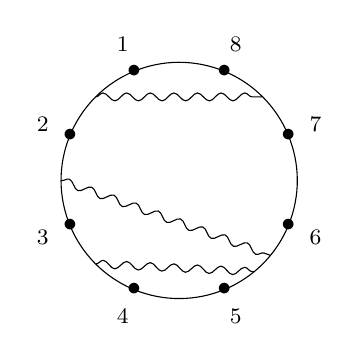
\begin{tikzpicture}[rotate=67.5,baseline=(current bounding box.east)]
	\begin{scope}
	\drawWLD{8}{1.5}
	\drawnumbers
	\drawprop{1}{0}{7}{0}
	\drawprop{3}{0}{5}{-1}
        \drawprop{2}{0}{5}{1}
		\end{scope}
	\end{tikzpicture}\eas and $W' = (\{(1,4), (3,5), (6,7), (8,1), (8,1)\}, [8])$ as \bas W'\ =\ 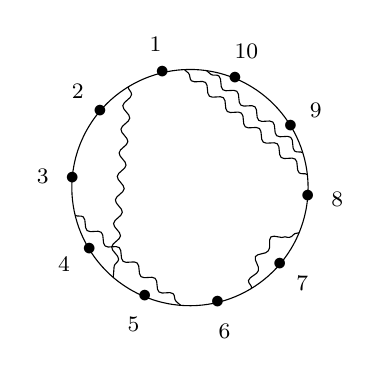
\begin{tikzpicture}[rotate=67.5,baseline=(current bounding box.east)]
	\begin{scope}
	\drawWLD{10}{1.5}
	\drawnumbers
	\drawprop{1}{0}{4}{0}
	\drawprop{3}{0}{5}{0}
        \drawpropbend{6}{0}{7}{0}{35}
	\drawprop{8}{1}{10}{-1}
 	\drawprop{8}{-2}{10}{2}
		\end{scope}
	\end{tikzpicture}\;.\eas 
Note that the pairs indicating the propagators are unorderer. That is if the propagator $p$ ends on the third and fifth edges, we may write $p = (3,5)$ or $p(5,3)$. In this paper, we use the convention that one may write $p = (i, j) = (j,i)$. That is, the two indices do not correspond to an ordered pair, or impose an orientation on $p$. Rather, they are simply the edges on which the propagators end. Furthermore, we use the convention that if two propagators have endpoints on the same edge, they are drawn so that they do not cross. 

In the diagram $W$, the propagators $p = (3,5)$ and $r = (2,5)$ both end on the the $5^{th}$  edge of the diagram. Therefore we say that these two edges are adjascent, and, when we need to refer to their positioning on the $5^{th}$ edge, refer to them as $q_1 = p$ and $q_2 = r$. Consider the set of these two propagators: $Q = \{p, r\}$. Then $V_Q = \{ 2, 3, 4, 5, 6\}$. Callthe remainining propagator in the diagram $s$: $s = (1, 7)$. Then $F(s) = \{1, 7, 8\} = V_Q^c$. In particular, the vertex $2$, which supports both $s$ and $r$, and therefore isn't an element of $F(s)$.
\end{eg}


In the physics literature, we are only intersted in a certain subclass of these graphs, called admissible Wilson loop diagrams. An \emph{admissible} Wilson loop diagram, $W = (\cP, [n])$ satisfies the following conditions:
\begin{enumerate}
\item \textbf{Non-crossing} No pair of propagators $p, q \in \cP$ cross in the interior of $W$. That is, for two propagaotors $p = (i,j), \; q = (k, l) \in \cP$ written such that $i <j$ and $k <l$ in natural linear order on $[n]$, if $i < k$ then $l <j$. 
\item \textbf{Local Density} Any subset of propagators $ P \subset \cP$ is supported by at least 3 more vertices than the number of propagators in $P$: $|V_P| \geq |P| + 3$. 
\item \textbf{Global Density} There are at least 4 more vertices in the diagram than there are propagators. That is $n \geq |\cP| + 4$.
\end{enumerate} 

Note that the diagram $W$ above is admissible, while $W'$ is not. Furthermore, note that local density implies that one cannot have a propagators $p = (i, i+1)$ or pairs of propagators with the same endpoints: $p = q = (i, j)$.

For the remainder of this paper, we restrict our attention only to admissible Wilson loop diagrams.


\subsection{Variable valued matrices and matroids \label{sec:matrices and matroids}}

Wilson loop diagrams have a natural matrix representation with real independent variable entries that bridges the combinatorics of the diagrams to matroids and to geometric subspaces of the positive Grassmannians. Before introducing this representation, we  define some notation around matrices with algebraically independent invertible variables, and recall some facts about Matroids

\begin{dfn} \label{dfn:variablevaluedmatrix}
Let $\cV = \{V_1, V_2, \dots, V_k\}$ be a collection of subsets of $\{1,2,\dots,n\}$. Let $\mathbf{x}=\{x_{i,j}\}$ be a set of algebraically independent invertible variables. Define $M_{\mathcal{V}}$ to be the $n \times k$ matrix having $x_{i,j}$ as its $i,j$ entry if $j \in V_i$ and $0$ otherwise.
\end{dfn}

One can realize a matrix $M_\cV$ at a point $\mathbf{x}=\{x_{i,j}\} \in \R^{|\mathbf{x}|}$ to get a real valued matrix. We can vary the points in $\R^{|\mathbf{x}|}$ to parametrize a family of real valued $k \times n$ matrices. Furthermore, by ignoring any such matrices of less than full rank, we may parametrize a subspact of $\Grall(k,n)$.

\begin{dfn} \label{dfn:loci}
Given a $k \times n$ variable valued matix $M_\cV \in M_{k,n}$, we write $L(\cV)$ to be the locus of the variables defining that matrix in $\Grall(k,n)$. In other words, $L(\cV)$ is the set of point of $\Grall(k,n)$ that can be realized by setting the entries of $M_\cV$ to real values.
\end{dfn}

The matrices of the form $M_\cV$ correspond to matroids \footnote{Specifically, they appear naturally transversal matroids \cite{????}, as disucssed in \cite{basisshapeloci}, but that is beyond the scope of this discussion.} For the remainder of this section, we give a brief overview of matroids, which the expert reader may skip. 

A matroid can be defined as a set, and a set of independence conditions on said set. For instance, one can define $M = (E, \mathcal{B})$, where $\mathcal{B}$, called a basis set, is a non-empty set of subsets of $E$, each of the same size, satisfying the basis exchange condition: \bas \textrm{for  all } A \textrm{ and } B \in \cB, \textrm{ if }  a \in A\setminus B \textrm{ then } \exists b \in B \setminus A \textrm{ and } (A \setminus a) \cup b \in  \cB \;.\eas Each element of $\mathcal{B}$ is a basis of $M$ and denotes a maximal independent set. The rank of the matroid, denoted $\rk(M)$ is the unique size of all the basis sets. We may also refer to the rank of a subset of $E$, $S \subset E$. We write the restriction of a matroid to $S$ $\rk(M|S) = \max \{B \subset S| B \in \mathcal{B} \}$, which, by abuse of notation, we also denote $\rk(S)$. 

Equivalently, one can define $M = (E, \mathcal{F})$, where $\mathcal{F} = \{ F \subset E| \forall x \in E \setminus F, \rk(F \cup x) > \rk(F)\}$ is the set of flats of $M$. For any subset $S \subset E$, we can define the closure of the set $\textrm{cl}(S)  = \{x \in E | \rk(S) = \rk(S \cup x)\}$ as the smallest flat containing $S$. Note that if $S$ and $T$ are two flats, then $S \cap T$ is also a flat. 

Also equivalently, we may write $M = (E, \mathcal{C})$ where $\mathcal{C} = \{C \subset E | \forall S \subsetneq C, \; S \subset B \textrm{ for some } B \in \mathcal{B}\}$ is the set of circuits of $M$. The circuits are the minimal dependent sets, i.e. each proper subset of $C$ is independent. If $C$ and $D$ are both circuits, then $C \cup D$ is a cycle. 

Given a matroid $M = (E, \mathcal{B})$, and a subset $S \subset E$, the restriction $M|S = (S, \mathcal{B|S} = \{B\cap S| B \subset \mathcal{B} \textrm{ such that } |B \cap S| \textrm{ maximal} \}$. The contration is defined $M/S = (E \setminus S, \mathcal{B/S} = \{B\setminus S| B \subset \mathcal{B} \textrm{ such that } |B \cap S| \textrm{ maximal}\}$. A matroid is disconnected if it can be written as the direct sum of two matroids: $M = (E_1, \mathcal{B}_1) \oplus (E_2, \mathcal{B}_2)  = (E_1 \cup E_2 , \mathcal{B}_1 \times \mathcal{B}_2)$. Otherwise, it is connected.

A matroid is representable if it can be written as a matrix with the same independence data. In particular, since the matrices $M_\cV$ have algebraically independent non-zero entries, it is straight forward to read off the matriod assoiciated to the collection of sets $\cV$.

\begin{eg}\label{eg:variablevaluesasmatroids}
Given a collection of subsets $\cV$ as in definition  \ref{dfn:variablevaluedmatrix}, we may define a matroid with a base set consiting of the columns of $M_\cV$. That is, $E = \{1, \ldots , n\}$. Then, a
for each subset $S \subset E$ define $\cV_S = \{V \in \cV | S \cap V \neq \emptyset\}$. That is $\cV_S$ is the set of rows of $M_\cV$ that have a non-zero entry in the columns indicated by $S$. In the matroid defined by $M_\cV$, the set $S$ is a cycle if $\cV_S$ contains strictly fewer elements than $S$. More informally, since the elements of $V$ correspond to rows of $M_\cV$, and the elements of $S$ its columns, this is simply saying that the set of columns $S$ are a dependent set if and only if there are fewer rows with non-zero entries than columns indicated by $S$. In the sequel, we will often abuse notation and refer to $M_\cV$ as both the matrix and the matroid it defines, and leave the distinction to be made from context.
\end{eg}


A positroid is a matroid, endowed with a cyclic ordering on the ground set, that can be realized as a matrix with all positive minors. Note that if $M$ is a positroid, as a matroid it is invariant under any cyclic permutation of the ground set. However, as a postroid, in order to  preserve the nonnegativity of the minors, it is only invariant under cycic permutations of the ground set. If a matroid is a positroid, then the cyclic ordering on $E$ defines a \hlfix{Gale ordering on the subsets}{Probably needs a definition or at least a cite?}. The minimal basis sets in this Gale ordering gives the Grassmann necklace associated to the positroid. 

One way to detemine if a matroid is a positroid is to look at its flacets. A flacet, $F$, of a (connected) matroid $M$ is any subset of $M$ such that $M|F$ and $M/F$ are both connected. If $M$ is a positroid, then every flacet is a cyclic interval. Furthermore, for any matroid, any flacet is a cyclic flat.

In this way, the word positroid has both a geometric meaning (as a subset of a Grasmannian) and a matroidal meaning (as a groundset where every flacet is a cyclic flat). These two meanings are tightly related in that every geometric positroid can be represented matroidally as a positroid and vice versa. When we refer to the matroid of a point in the positive Grassmanians, we refer to the positroid of that point in the matroidal sense. When we say the positroid of a matrix, we refer to the geometric meaning. \sanote{make this clearer?}

\section{Geometry of Wilson loop diagrams \label{sec:WLDgeom}}

We are now ready to apply the notation above to Wilson loop diagrams. We first show that a Wilson loop diagram can be associated to a matrix with real independent variable entries. 

In order to associate a matrix to a Wilson loop diagram, $W = (\cP, [n])$,  to each propagator $p \subset \cP$ associate a $4$ dimensional subspace of $\RP^{n+1}$ of the form \bas Y_p = \begin{cases}  x_{p,i} &  i = 0 \textrm{ or } i \in V_p \\ 0 &  \textrm{else,}\end{cases} \eas where $x_{p,i}$ are algebraically independent real valued variables \cite{a physics paper}.Then one may associated to $W$ a subspace of $\Grall(k, n+1)$ given by the linear span of the $Y_p$. 

In otherwords, for each Wilson loop diagram $(\cP, [n])$, we have two sets of subsets \bas \YP = \{ V_p \cup 0 | p \in \cP\} \quad \textrm{ and } \quad \VP = \{ V_p | p \in \cP\} \eas  that define two matrices $M_{\VP}$ and $M_{\YP}$. These define subspaces of $\Grall(k, n+1)$ and $\Grall(k, n)$ respectively, that we call $L(\YP)$ and $L(\VP)$ as in Definition \ref{dfn:loci}.

\begin{eg} \label{eg:matrices}That is, given the Wilson loop diagram $W$ in example \ref{eg:admissible}, with $p = (3,5)$, $r = (2,5)$, and $s = (1,7)$ one may write \bas M_{\YP} = \begin{bmatrix}  x_{p,0} & 0 & 0 &x_{p,3} & x_{p,4} &  x_{p,5} & x_{q,6} & 0 & 0 \\ x_{r,0} & 0 & x_{r,2} & x_{r,3} & 0  &x_{r,5} & x_{r,6} & 0 &0 \\ x_{s,0} & x_{s,1} & x_{s,2} & 0 &0 &0 &0 &x_{s,7} & x_{s,8} \end{bmatrix} \;.\eas

We define the matrix $M_{\VP}$ to be the one defined by ignoring the first column of $M_{\YP}$.  In the running example, \bas M_{\VP} = \begin{bmatrix}  0 & 0 &x_{p,3} & x_{p,4} &  x_{p,5} & x_{q,6} & 0 & 0 \\ 0 & x_{r,2} & x_{r,3} & 0  &x_{r,5} & x_{r,6} & 0 &0 \\  x_{s,1} & x_{s,2} & 0 &0 &0 &0 &x_{s,7} & x_{s,8} \end{bmatrix} \;.\eas
\end{eg}

 
\begin{rmk}
Note that, as a subspace of $\Grall(k, n)$ (resp. $\Grall(k, n+1)$), or ordering of the rows in $M_{\VP}$, resp. $M_{\YP}$ do not matter.
\end{rmk}

\begin{rmk}
It is also worth noting that in previous literature, the matrices $M_{\YP}$ and $M_{\VP}$ were denoted $C_*(W)$ and $C(W)$ respectively. However, in this paper, we wish to exploit the results of \cite{basisshapeloci} to understand the properties of the parametrized spaces, and therefore, change the naming conventions. 
\end{rmk}

\subsection{Wilson loop diagrams as positroids \label{sec:WLDmatroid}}

In \cite{wilsonloop} the authors show that each admissible Wilson loop diagram is assoicated to a positroid, which we also call $M_\cV$, or a matroid that can be represented by a matrix with positive maximal minors. In other words, the loci $L(\VP) \subset \Grall(k,n)$ intersects the positive Grassmannian, $\Gr(k,n)$. Positroid varieties give a tiling of $\Gr(k,n)$ into positroid cells \cite{??}, which we refer to by the letter $\Sigma$. In \cite[Theorem 8.4]{basisshapeloci} the author shows that for a Wilson Loop diagram $W = (\cP, [n])$, the closure of the intersection of the locus wtih the positive Grassmannian corresponds to the closure of a postroid cell in that positive Grassmanian: $\overline{L(\VP) \cap \Gr(k,n)} = \overline{\Sigma(\VP)}$. In this section, we discuss the relationship between Wilson loop diagrams and postroids. In section \ref{sec:geometry}, we discuss their geometry as a subset of $\Grall(k, n)$. We begin with a brief summary of the matroidal properties of Wilson loop diagrams, we give a brief overview of matroids and positroids. Those familiar with the subject may skip the followins section.


\subsubsection{Wilson Loop diagrams as matroids} 
The matroidal properties of Wilson loop diagrams derived in \cite{Wilsonloops}  can be verified by considering the independent columns of $M_{\VP}$.
\begin{enumerate} 
\item Theorem [3.9] of \cite{wilsonloops} states that a set of vertices of a Wilson loop diagram, $(\cP, [n])$  is independent if and only if no subset supports fewer propagators than vertices in the subset. I.e. $V \subset [n]$ is independent if, for all $U \subseteq V$, $\Prop(U) \geq |U|$. In terms of rows and columns of $M_{\VP}$, this simply states that any set of columns of $M_{\VP}$ contains a dependent subset if said subset is non-zero on fewer rows than columns in the subset.
\item Corrollary [3.39] shows that all admissible Wilson loop diagrams, in particular those satisfying the non-crossing and local density conditions, correspond to positroids. This means that, as matroids, the Wilson loop diagrams can be represented by matrices with all positive maximal minors. That is, the subspace of $\Grall(k,n)$ parametrized by $M_{\VP}$ intersects $\Gr(k,n)$.
\end{enumerate}


\begin{eg}\label{eg:wldmatroid}The independence condition in \cite[Theorem 3.9]{wilsonloops} is equivalent to saying that $U$ is a cycle of the matroid associated to $W$, call it $M_{\VP}$, if and only if  $|\Prop (U)| \leq |U|$. This is exactly the same as the cycle condition laid out in Example \ref{eg:variablevaluesasmatroids}. For instance, in $W$  from Example \ref{eg:admissible}, the vertices $\{7,8\}$ are a cycle since they only support one propagator between them. In fact, the define a circuit. On the other hand, the vertices $\{3,4\}$ support two propagators, and thus are independent. Consider the set of proppagators $P = \{ (2, 5), (3, 5)\}$. Then $F(P) = \{ 1, 7, 8\}$. This is a flat of rank $2$. In \cite{wilsonloops}, set of the form $F(P)$ are called propagator flats, and the author shows that the cyclic flats of the matroid assoicated to $W$ are propagator flats.
 \end{eg}


\subsubsection{Geometry of WLDs \label{sec:geometry}}
Paralell to the the conventions of \cite{casestudy, generalcombinatorics1}, we call the positroid cell defined by the Wilson loop diagram $(\cP, [n])$, $\Sigma(\VP)$. We indicate by $\cW_{k,n}$ be the set of all admissible Wilson loop diagrams with $k$ propagators and $n$ vertices. In \cite[Theorem 8.4]{basisshapeloci}, the author shows that $\overline{L(\VP) \cap \Gr(k,n)} = \overline{\Sigma(\VP)}$. In other words, the space $L(\VP)$ differs from the positroid cell $\Sigma(\VP)$ only on a set of measure 0. For an explict example of where these spaces differ, see Example \ref{eg:closuresmatch}. The author of \cite{basisshapeloci} also shows each $\Sigma(\VP)$ is a $3k$ dimensional cell. More generally, the author shows, using slightly different notation:

\begin{thm}[Theorem 3.2, \cite{basisshapeloci}]\label{res:minimalrep}
Given a variable valued $k \times n$ matrix $M_\cV$ with $m$ non-zero entries representing a positroid cell $\Sigma(\cV)$, the following are equivalent:
\begin{enumerate}
\item $\dim(\Sigma(\cV)) = m -k$ 
\item $M_\cV$ has the smallest number of non-zero variable entries of any variable valued matries representing $\Sigma(\cV)$
\item For all $\mathcal{T} \subseteq \cV$, \bas |\bigcup_{T \in \mathcal{T}}T| \geq \max_{T \in  \mathcal{T}} (|T|) + |\mathcal{T}| -1 \;. \eas
\end{enumerate}
\end{thm}


In \cite[section 2.3]{non-orientable}, the authors show that  the subspace of $\Grall(k,n)$ parameterized by $M_{\YP}$, can be viewed as a real $k$ vector bundle over the space parametrized by $M_{\VP}$, i.e.  $\cup_{W \in \cW_{k,n}}L(\YP) \rightarrow \cup_{W \in \cW_{k,n}}L(\VP)$. Restricting to any given Wilson loop diagram gives a trivial vector bundle $L(\YP) \rightarrow L(\VP)$. As shown in Theorem 2.29 of loc. cit., the space $\cup_{(\cP, [n]) \in \cW_{k,n}}L(\YP)$ need not be orientable. 

\begin{rmk} \label{rmk:parametrization} We have now constructed a map from Wilson loop diagrams to the positroid cells. First note that every diagram $W = (\cP, [n])$  defines a map between products of projective spaces: \ba  \xymatrix{(\RP^4 )^{\times k}  \ar@{^{(}->}[r]^-{W} &  \{Y_p | p \in \cP\} \subset (\RP^{n+1} )^{\times k}  } \;. \label{eq:maps}\ea When the set of vectors $\{Y_p | p \in \cP\}$ are in general position, they define a $k$-dimensional hyperplane in $\RP^{n+1}$. Thus, outside of a space of measure $0$, the vectors $\{Y_p | p \in \cP\}$ parametrize a subspace of $\Grall(k,n+1)$, which we call $L(\YP)$. At the same time the parametrized sapces define a vector bundle: $L(\YP) \rightarrow L(\VP)$. In \cite{wilsonloops}, the authors show that the matroid defined by $M_{\VP}$ is a positroid, i.e. it intersects the non-negative Grassmannian. Furthermore, \cite{basisshapeloci} shows that \ba \overline{L(\VP) \cap \Gr(k,n)} = \overline{\Sigma(\VP)} \label{eq:density}\ea where $\Sigma(\VP)$ is the positroid cell in $\Gr(k,n)$ defined by the positroid $M_{\VP}$. In other words, up to a space of measure $0$, the spaces parametrized by the Wilson loop diagrams, $\{Y_p\} \subset (\RP^{n+1})^k$ and $M_{\VP} \subset (\R^{n \times k}$ also parametrize positroid cells in the positive Grassmannians. \end{rmk} \todo{put in theorem numbers}


{\color{red} Got rid of this display in the above discussion: \bas \overline{\textrm{span}\langle\{Y_p | p \in \cP\}\rangle} = L(\YP)\;. \eas Are we okay with that?}

%The composition of the first two maps comes from the definition of the vectors $Y_p$.  The map $\cup_{W \in \cW_{k,n}}L(\YP) \rightarrow (\RP^{n+1} )^{\times k}$ is formed by setting the first entry of each $Y_p$ to 1. (Note, that in making this choice, we are deliberately preventing the variables in the first column of $M_{\YP}$ from being $0$. In the physics literature, these points correspond to the physical poles of the scattering amplitude \cite{}, and therefore are not the subject of this paper.) Under this choice, it is a dense inclusion for each $W \in \cW_{k,n}$. \sanote{this paragraph is too central to our arguments to leave like this. Can we specify it better?}


\subsection{Integrals and poles \label{sec:integrals}} \todo{divide into 2 sections? maybe before Theorem 3.8?}

The goal of this paper is to show that the spurious poles of the Wilson loop diagrams cancel in the calculation of the full amplitude. Recall that there are two types of singularities to this theory: the physical poles and the spurious poles. The physical poles arise when the vectors representing the particles do not span $\R^4$, as one expects in a physical theory with infrared singularites. The sprurious poles are those that arise in each summand of the integrals involved in calculating the three level scattering amplitude. These should cancel in the sum. In this section, we discuss the algebraic and geometric propoerties  of these poles. 

The Wilson loop diagrams represent the tree level contributions to the scattering amplitudes in the physical theory N=4 SYM. The holomorphic Wilson loop for $n$ particles and $k$ propagators gives the contribution to the n particle scattering amplitude of N=4 SYM by $k$ propagators. The tree level contribution to this amplitude is given by a sum of integrals associated to admissible Wilson loop diagrams: \ba \cA_{k,n}^{tree} = \sum_{(\cP, [n]) \subset \cW_{k,n}} I(\VP) \;.\label{eq:treelevelamplitude}\ea The scattering amplitude is a functional on the particles of the theory, represented in twistor space. In this case, the external data are represented as $n$ sections of a $k$ dimensional real vector bundle over a real twistor space, $\{Z_1, \ldots, Z_n\}$  such that the $n \times n+4$ matrix who's $i^{th}$ row is $Z_i$ has positive maximal minors. Furthemore, we fix a guage section, $Z_0$, which can be taken, without loss of generality to be a $0$ section. We define the matrices \bas \cZ = \begin{bmatrix} - & Z_1& - \\ & \vdots &  \\ - & Z_n& -\end{bmatrix} \; ; \; \cZ_* = \begin{bmatrix}- & Z_0& - \\  - & Z_1& - \\ & \vdots & \\  - & Z_n& -\end{bmatrix} \; .\eas Note from above, the matrix $\cZ$ has positive maximal minors, while the matrix $\cZ_*$ may not.

Before we define the actual integral, $\cI(\VP)$, recall that if multiple propagators end on the $e^{th}$ edge, we order them according to their proximity to the vertex $e$. We are now ready to define the integrals assoicated to each Wilson loop diagram $W = (\cP, [n])$, with $k = |\cP|$:

\begin{dfn} \label{dfn:I(W)} \bas \cI(\VP) (\cZ_*)  = \int_{(\RP^4)^k} \frac{\prod_{p \in \cP} \prod_{v \in V_p} dx_{p, v}}{R(\VP)} \delta^{4k|4k}(M_{\YP} \cdot \cZ_*) \eas where, for $X$ a $k \times k+4$ matrix, \bas \delta^{4k|4k}(X) = \prod_{b =1}^k (X_{b, 4+b})^4\delta^4((X_{b,1},X_{b,2},X_{b,3},X_{b,4}))  \eas and $R(\VP)$ is a polynomial determined from the $W$ as follows: 
\begin{enumerate}
\item Define $R_e = x_{q_1, e+1} \big(\prod_{r = 1}^{s-1} (x_{q_r, e}x_{q_{r+1}, e+1} - x_{q_r, e+1}x_{q_{r+1}, e})\big) x_{q_s, e}$
\item $R(\VP) = \prod_{e \in [n]} R_e$
\end{enumerate} \end{dfn}

There are a few features to note in this defintion. First, notice that the spurious poles of the theory correspond to setting the factors of $R(\VP)$ to zero. Specifically, by equations \eqref{eq:matrixvalues} in Appendix \ref{sec:appendix}, the variables $x_{p,0}$ localize to $0$ when the vectors representing the particles do not span $\R^4$. This corresponds to the physical poles of the theory. The spurious poles occur when  $x_{p,0} \neq 0$, but the polynomial $R(\VP)$ goes to $0$. See \cite{casestudy, HeslopSteward, AmplituhedonSquared} for more calculations of this form. 

Secondly, note that in this definition, we take the integral over $(\RP^4)^k$, while previously, we have referred to the matrices as parametrizing subspaces of $\Gr(k,n)$. This is permissible due to the density arguments following display \eqref{eq:maps}. Namely, the integal $I(\VP)$ is defined on all but the set of measure 0 where $M_{\YP}$ is of less than full rank. This subspace is exactly $L(\YP)$, which differs from $\Sigma(\VP) \times \R^k$ by a set of measure 0. 

Equation \eqref{eq:treelevelamplitude} shows that $N^kMHV$ (tree level) amplitude
on $n$ points is taken to be the sum of all the integrals associated
to tree level Wilson loop diagrams. Theorem \ref{res:polesonboundaries} shows that the spurious poles
all fall on the boundaries of a geometric space defined by these diagrams. In Theorem \ref{res:deg1polescancel} we show that
the poles that fall on codimension 1 boundaries cancel. However, unlike in the
Amplituhedron story, one cannot assoiciate a geometric meaning to the
sum of these integrals. In \cite{non-orientable}, the authors show
that while the subspace of $\Grall (k,n+1)$ associated to each
$M_{\YP}$ is orientable, the union of said spaces are not. Therefore,
one cannot interpret the sum of the associated integrals as the volume
of a geometric space. This result has also been shown explicitly and
separately in \cite{HeslopStewart} which explicitly calculates a contradiction that
occurs if one attempts this interpretation.

Here, we propose a different geometric interpretation of the sum of
these integrals. One can consider $\overline{L(\YP)}$ as the closure of a $k$-dimensional
  line bundle over $\overline{L(\VP)}$ \cite{non-orientable}. Then, we may consider the
cancelation of spurious poles on any section of the bundle, i.e. after fixing values to the variables $x_{p, 0}$. In fact,
for the spurious poles, one typically sets the values of $x_{p,0}$ to
be $\pm 1$, and factors of $R(\VP)$ evaluates to $0$ \cite{??}. The physical poles of the tree level amplitude $A_{k,n}$ arise when the variables $x_{p, 0} = 0$. 

In \cite{GWLDCII}, the authors show a direct relationship between the polynomial $R(\VP)$ and the positroid cell $\Sigma(\VP)$. They show that the prime factors of $R(\VP)$ to are also the prime factors of the product of the minors defined by the Grassmann necklace of $\Sigma(\VP)$. We restate it here using the notation of this paper.

\begin{thm} \cite[Proposition 5.3]{GWLDCII} \label{res:prop alg gives rad}
Write $\cI = \{I_1, \ldots I_n\}$ be the Grassmann necklace assoicates to the positroid cell $\Sigma(\VP)$. Let $\Delta_{I_i}$ be the minor of $M_{\VP}$ defined by the columns indicated by $I_i$. Then
  \begin{enumerate}
   \item Each $\Delta_{I_i}$ splits into linear and quadratic factors.  All linear factors of  $\Delta_{I_i}$ are single variables and all irreducible quadratic factors are $2\times 2$ determinants of single variables.
    \item Quadratic factors in $\Delta_{I_i}$ arise precisely when propagators $p$ and $q$ are supported on a common edge $a$ with $I_i(p)=a$ and $I_i(q)=a+1$.
    \item The factor $r_e$ divides $\Delta_{I_e}$.
    \item The ideal generated by $R(\VP)$ is the radical of the ideal generated by $\prod_{i=1}^{n}\Delta_{I_i}$.
  \end{enumerate}
\end{thm}

We can generalize this result to define a polynomial given by a minimal parametrization of a positroid cell. 

\begin{dfn}\label{dfn:RV}
Let the set of subsets $\cV$ define a matroid $M_{\cV}$. If $M_{\cV}$ is also a positroid, let $\cI =  \{I_1, \ldots I_n\}$ be the associated Grassman Necklace. Then define $R(\cV)$ be the polynomial formed by the product of the prime factors of $\prod_{i=1}^{n}\Delta_{I_i}$. That is, $R(\cV) = \textrm{rad}(\prod_{i=1}^{n}\Delta_{I_i})$. 
\end{dfn}

\begin{eg} \label{eg:differentpolys} Note that the polynomial $R(\cV)$ is dependent on the minimal parametrization of the postroid defined by $\cI$. For instance, in \cite{GWLDCI}, the authors give conditions for when multiple Wilson loop diagrams can correspond to the same positroid cell. For example both $\cV_1 = \{\{1, 2, 4, 5\}, \; \{1, 2, 3, 4\} \}$ and $\cV_2 = \{\{1, 2, 4, 5\}, \; \{2, 3, 4, 5\} \}$ define the same matroid. However \bas R(\cV_1) = x_{1,2}(x_{1,1}x_{2,2}- x_{2,1}x_{1,2})x_{2,1}x_{2, 3}x_{2,4}x_{1,4}x_{1,5}  \quad \textrm{while} \\ R(\cV_2) =  x_{1,1}x_{1,2}x_{2,2}x_{2, 3} x_{2,5}(x_{1,4}x_{2,5}- x_{2,4}x_{1,5})x_{1,4}\;.\eas Both correspond to the polynomial formed by the product of the prime factors of $\prod_{i=1}^{n}\Delta_{I_i}$ under the corresponding coordinate system. \end{eg}

In this paper, we are interested in the poles of $I(\VP)$ that lie on codim 1 subspaces of $\overline{\Sigma(\VP)}$. By construction, these are the factors of $R(\VP)$ that have vanishing loci on codim 1 subspaces of $\overline{\Sigma(\VP)}$. Proposition \ref{res:vanishonbdny} shows that all factors of $R(\VP)$ vanish on the boundary of $\Sigma(\VP)$. Then, Theorem \ref{res:polesonboundaries} shows that if the vanishing loci has codimension 1, then it is dense in some codimension $1$ boundary of $\Sigma(\VP)$, and Theorem \ref{res:deg1polescancel} shows that the all the poles with codimension 1 vanishing loci cancel in the sum  $A_{k,n}$ cancel. 

In order to do this, we to show that the factors of $R(\VP)$ vanish on the boundary of the associated positroid cells. In \cite{generalcombinatoricsII}, the authors show that $R(\VP)$ is exactly the product of the prime factors of the determinants of $M_{\VP}$ defined by the Grassmann necklace of the associated matroid, $\Sigma(\VP)$. Then we show that when the factor of $R(\VP)$ corresponds to a simple pole in the integral (i.e. a codimension 1 boundary of $\Sigma(\VP)$), the locus of the resulting matrix is dense in the corresponding boundary cell in the Grassmannian.

\todo{pick up here}

\begin{prop}\label{res:vanishonbdny}
All the factors of $R(\VP)$ vanish on the boundary of $\Sigma(\VP)$.
\end{prop}


\begin{proof}
Let $\{I_1, I_2, \dots, I_k\}$ be the Grassmann necklace associated $\Sigma(\VP)$. From Proposition 5.3 in \cite{generalcombinatoricsII},
%
\begin{displaymath}
R(\VP) = \mathrm{rad}\left(\prod_{i = 1}^{k} \Delta_{I_i}\right).
\end{displaymath}
%
From Theorem 5.15 in \cite{knutsonlamspeyerjuggling}, the ideal of functions defining the variety $\overline{\Sigma(\VP)}$ is generated by $\{\Delta_I : I \notin M(W)\}$. From (THEOREM NUMBER) in \cite{basisshapeloci}, $G(W) \subset \overline{\Sigma(\VP)}$ and hence every function vanishing on $\Sigma(\VP)$ vanishes on $G(W)$. Theorem 5.1 in \cite{knutsonlamspeyerjuggling} implies that the open positroid variety $\Sigma(\VP)$ is defined as a subset of $\overline{\Sigma(\VP)}$ by
%
\begin{displaymath}
\Delta_{I_1}, \Delta_{I_2}, \dots, \Delta_{I_k} \neq 0.
\end{displaymath}
%
Thus, the subset of $G(W)$ where $R(\VP)$ vanishes is exactly
%
\begin{displaymath}
G(W) \setminus \Sigma(\VP) \subset \overline{\Sigma(\VP)} \setminus \Sigma(\VP). \qedhere
\end{displaymath}
\end{proof}

\begin{eg} \label{eg:closuresmatch}
This example illustrates the differences between the sets $G(W)$, $\Sigma(\VP)$, and $\overline{\Sigma(\VP)}$. Let
\bas M_{\VP} =
\begin{bmatrix}
x_{p,1} & x_{p,2} & 0 &x_{p,4} & x_{p,5} & 0 \\
x_{q,1} & x_{q,2} & 0 & 0 & x_{q,5} & x_{q,6}
\end{bmatrix}.\eas
\noindent
Let $\Sigma(\VP)$ and $\overline{\Sigma(\VP)}$ be the associated open and closed positroid cells respectively.

The point represented by
\begin{displaymath}
\begin{bmatrix}
1 & 1 & 0 & 1 & 1 & 0 \\
1 & 1 & 0 & 0 & 1 & 1
\end{bmatrix}
\end{displaymath}
\noindent
is in $G(W) \setminus \Sigma(\VP)$, since the minor $\Delta_{I_1} = \Delta_{12}$ vanishes. Hence,
%
\begin{displaymath}
R(\VP) = (x_{p,1}x_{q,2} - x_{p,2}x_{q,1}) x_{p,1} x_{p,4} x_{p,5} x_{q,2} x_{q,5} x_{q,6}
\end{displaymath}
\noindent
vanishes at this point.

The point represented by
\begin{displaymath}
\begin{bmatrix}
1 & 0 & 0 & 1 & 0 & 1 \\
0 & 1 & 0 & 1 & 1 & 1
\end{bmatrix}
\end{displaymath}
\noindent
is in $\Sigma(\VP) \setminus G(W)$ since there is no point in $G(W)$ where $\Delta_{45},\Delta_{56} \neq 0$ and $\Delta_{46} = 0$.

The point represented by
\begin{displaymath}
\begin{bmatrix}
0 & 0 & 0 & 0 & 1 & 0 \\
0 & 0 & 0 & 0 & 0 & 1
\end{bmatrix}
\end{displaymath}
\noindent
is in $\overline{\Sigma(\VP)} \setminus \Sigma(\VP) \cup G(W)$.
\end{eg}

This fact has been shown explicitly in the case of $n = 6$ and $k=2$, however, has not been shown in general.

Next we show that the loci of the matrices after the codimension 1 poles of $R(\VP)$ have been set to 0 is dense in the corresponding positroid.

\todo{Check if the closures of Loci are put in the right places throughtout paper}

\begin{thm}\label{res:polesonboundaries}
Let $W=(\mathcal{P},[n])$ be an admissible Wilson loop diagram and let $L' \subset L(\VP)$ be the vanishing locus of a single factor of $R(\VP)$ inside $L(\VP)$ and suppose that $L'$ has codimension $1$ in $L(\VP)$. Then, $\overline{L'\cap \Gr(k, n)} = \overline{\Sigma'}$, where $\Sigma'$ is a positroid cell in the boundary of $\Sigma$. \end{thm}

\begin{proof}
From CITE THEOREM, $R(\VP)$ is the product of individual entries and two by two minors of $M_{\mathcal{P}}(\mathbf{x})$. Suppose first that $G'$ is a codimension $1$ boundary obtained by setting a single variable $x_{p,i}$ to zero. Then, $G'$ is the subset of the Grassmannian consisting of row spaces of matrices of the form $M_{\mathcal{P}}(\mathbf{x})$ where $x_{p,i}$ is set to zero and all other entries are evaluated at real numbers. Theorem CITE THEOREM implies that a generic point in $G'$ represents the same matroid. Since the positroid stratification is coarser than the matroid stratification, a generic point in $G'$ is contained in the closure of some positroid $\Sigma' \subset \overline{\Sigma}$. Proposition \ref{res:vanishonbdny} implies that $G' \subset \overline{\Sigma} \setminus \Sigma$ and so $\Sigma' \neq \Sigma$. Since $G'$ was assumed to be codimension $1$, the matroid represented by a generic point in $G'$ is in fact $\Sigma'$. Then, Theorem CITE THEOREM implies that $\overline{G'} = \overline{\Sigma'}$, as desired.

Next, suppose that $G'$ is a codimension $1$ boundary obtained by setting a two by two minor of $M_{\mathcal{P}}(\mathbf{x})$ to zero. As in Lemma \ref{lem:simplifyR(W)}, $G'$ may be represented by reparameterizing this two by two minor in $M_{\mathcal{P}}(\mathbf{x})$, then setting one of the new parameters to zero. Let $M'$ denote the matrix obtained by this operation. Generic points in $G'$ represent the same matroid, namely the matroid whose bases are the minors $M'$ which aren't identically zero. Proposition \ref{res:vanishonbdny} implies $G' \subset \overline{\Sigma} \setminus \Sigma$. Then, since $G'$ has codimension $1$ in $\overline{\Sigma}$, the matroid represented by a generic point in $G'$ is a positroid $\Sigma'$. The open positroid $\Sigma'$ has a parameterization via a Marsh-Reitsch matrix $R$ in the same number of variables as $M'$. Then, as in the proof of CITE THEOREM, $M'$ and $R$ are generically related by a change of basis matrix and thus $\overline{G'} = \overline{\Sigma'}$.
\end{proof}

\begin{eg} \label{eg:codim2}
Note that not all factors of $R(\VP)$ correspond to codimension 1 subspaces of $\Sigma(\VP)$. 

For instance, consider the diagram in Example \ref{eg:closuresmatch}. Setting $x_{p,4}$ to $0$ gives the matrix \bas C' =
\begin{bmatrix}
x_{p,1} & x_{p,2} & 0 &0 & x_{p,5} & 0 \\
x_{q,1} & x_{q,2} & 0 & 0 & x_{q,5} & x_{q,6}
\end{bmatrix}, \eas which can be written as $M_{\cV}$ with $\cV = \{V_1 = \{ 1, 2, 5\}, V_2 = \{1, 2, 5, 6\}\}$. Note that while $ |\bigcup_{V \in \cV}V|  = 4$,
\begin{displaymath}
\max_{V \in  \cV (|V|)} + |\cV| -1  = 4 + 2 - 1.
\end{displaymath}
Therefore the third equivalent statement of Theorem \ref{res:minimalrep} does not hold, and thus $M_{\cV}$ is not parametrize a $5$ dimensional subspace of $\Gr(k,n)$. Since, by display (1) of \cite{basisshapeloci}, $5$ was an upper bound on the dimension of $L(\cV)$, setting $x_{p,4}$ must correspond to a higher codimension subspace of $\Sigma(\VP)$. 

\end{eg}

We show in section \ref{sec:boundarysanspoles} that the converse of Theorem \ref{res:polesonboundaries} does not hold. Namely, not every co-dimension one boundary of $\Sigma(\VP)$ contains the vanishing loci of a factor of $R(\VP)$.  \sanote{we really need to set a notation that explains that we are only referring to the vanishing loci in the positive Grassmanninas, so we don't have to keep saying it.}


\section{The poles of Wilson loop diagrams \label{sec:poles}}

\subsection{Cluster algebras, frozen variables, Grassmann Necklaces \label{sec:clusteralgebras}}

As a brief aside, we note that the polynomial $R(\VP)$ has appeared in relation to a cluster algebra associated to the positroid $\Sigma(\VP)$. Let $\mathcal{I} = \{I_1,I_2, \dots, I_k\}$ be the Grassmann necklace associated to $\Sigma(\VP)$. So, $I_j$ is that minimal set in the $j^{th}$ cyclic shift of the Gale order on sets such that the Pl\"ucker coordinate $\Delta_{I_j}$ is non-vanishing on $\Sigma(\VP)$. Let $\mathcal{I}^{\ast} = \{I^{\ast}_1, I^{\ast}_2, \dots, I^{\ast}_{k}\}$ be the reverse Grassmann necklace associated to $\Sigma(\VP)$. That is, $I^{\ast}_j$ is that maximal set in the $j^{th}$ cyclic shift of the Gale order on sets such that the Pl\"ucker coordinate $\Delta_{I^*_j}$ is non-vanishing on $\Sigma(\VP)$. Following Chapter 5 of \cite{knutsonlamspeyerjuggling} replacing Schubert varieties in the Grassmannian with reverse Schubert varieties, one sees $\Sigma(\VP)$ can equivalently be defined as an intersection of reverse Schubert varieties. Running the combinatorial algorithm for {\color{red} citation?} produces a Grassmann necklace for $\Sigma(\VP)$ given the diagram $W$ in clockwise, rather than counter clockwise, order yields the reverse Grassmann necklace for $\Sigma(\VP)$. Define
%
\begin{displaymath}
R^{\ast}(W) = \mathrm{rad}\left(\prod_{i = 1}^{k} \Delta_{I^{\ast}_i}\right).
\end{displaymath}

%{\color{red} the paragraph above might have been kind of fast, but i think it gives enough to convince the reader of the following lemma we had been including? at least enough for an aside section?

%\begin{lem}
%We can read the backwards GN off the diagram by reversing direction. 
%\end{lem}}


\begin{thm}
Using the notation from above, $R^{\ast}(W) = R(\VP)$.
\end{thm}

\begin{proof}
This follows from the fact that $R^{\ast}(W)$ and by $R(\VP)$ are both radical polynomials defining the same subvariety of the Wilson loop cell $G(W)$. 

From Section 5 of \cite{knutsonlamspeyerjuggling}, the open positroid variety $\Sigma(\VP)$ is defined as a subset of $\overline{\Sigma(\VP)}$ by $\Delta_I \neq 0$ for all $I \in \mathcal{I}$, where $\mathcal{I}$ is the Grassmann Necklace of $\Sigma(\VP)$. So, $\prod_{I \in \mathcal{I}} \Delta_I$ defines the subvariety $(\overline{\Sigma(\VP)} \setminus \Sigma(\VP)) \subset \overline{\Sigma(\VP)}$, the boundary of the open positroid inside the closed positroid. 

Let $G(W)$ be the geometric space parameterized by the Wilson Loop diagram $W$. From Theorem ?? in \cite{basisshapeloc}, $G(W) \subset \overline{\Sigma(\VP)}$. Let $V$ be the subset of $G(W)$ which is the pull back of the set in $(\mathbb{RP}^{4})^{k}$ where $R(\VP)$ vanishes via (\ref{eq:maps}). Then,

%
\begin{equation} \label{eqn:rw_vanishes}
\begin{split}
V & = V \cap \overline{\Sigma(\VP)} \\
& = G(W) \cap (\{\Delta_I = 0 : \exists I \in \mathcal{I}\} \cap \overline{\Sigma(\VP)}) \\
& = G(W) \cap (\overline{\Sigma(\VP)} \setminus \Sigma(\VP)) \\
& = G(W) \setminus \Sigma(\VP).
\end{split}
\end{equation}

Theorem ?? from \cite{generalcombinatorics2} shows that $R(\VP)$ generates the radical of the ideal generated by $\prod_\mathcal{I} \Delta_{I_i}$.

Following Section 5 of \cite{knutsonlamspeyerjuggling} replacing Schubert varieties with opposite Schubert varieties, $\Sigma(\VP)$ is similarly defined as a subset of $\overline{\Sigma(\VP)}$ by $\Delta_{I^{\ast}} \neq 0$ for all $I^{\ast} \in \mathcal{I}^{\ast}$. So, $\prod_{I^{\ast} \in \mathcal{I}^{\ast}} \Delta_{I^{\ast}}$ also defines the subvariety $(\overline{\Sigma(\VP)} \setminus \Sigma(\VP)) \subset \overline{\Sigma(\VP)}$. Following (\ref{eqn:rw_vanishes}), the pull back of the vanishing set of $R^{\ast}(W)$ from $(\mathbb{RP}^4)^{k}$ to $\Grall(k,n)$ is also $G(W) \setminus \Sigma(\VP)$. Pulling this set back to $(\mathbb{RP}^4)^{k}$, polynomials $R(\VP)$ and $R^{\ast}(W)$ vanish on the same set. $R^{\ast}(W)$ is radical by definition. Since $R^{\ast}(W)$ and $R(\VP)$ are radical polynomials defining the same variety, $R^{\ast}(W) = R(\VP)$.
\end{proof}


\begin{rmk}
Be careful that above $R(\VP)$ and $R^{\ast}(W)$ are both polynomials in the matrix entries $x_{p,i}$. The radicals taken are over the polynomial ring in these variables, defining a variety in the space of $n \times k$ matrices. To pass to the Grassmannian and obtain the variety $\overline{\Sigma(\VP)}$, one must further remove singular matrices and quotient by the left action of $\mathrm{Gl}(k)$. 
\end{rmk}

{\color{red} finally, have a paragraph just saying what role $R^{\ast}(W)$ plays in the cluster algebra stuff (at least as well as i understand it)}

%\begin{thm}
%If a WLD does not have a non-trivial exact subdiagram, then $M_{\VP}$ is its unique  minimal representation. {\color{red} Again, do we need this?...i don't think we need this for this section?}
%\end{thm}

\subsection{Geometry of the poles\label{sec:boundarysanspoles}}

Note that not every co-dimension one boundary of a $\Sigma(\VP)$ contains the vanishing loci of a factor of $R(\VP)$. In order to reach a boundary of a positroid cell, one must send certain minors to 0 while not causing any perviously vanishing minors to become positive. Sending parameters to $0$, which causes the polynomial $R(\VP)$ to vanish, is certainly one way to do this. However, the boundary of $\Sigma(\VP)$ contains other positroid cells which do not necessarily intersect the vanishing set of $R(\VP)$. In this section, we give one criterion for identifying boundaries of positroid cells that do not contain the loci of these vanishing factors. 

We begin with an example. 

\begin{eg} \label{eg:strangeboundary}
The Wilson loop diagram\bas W =  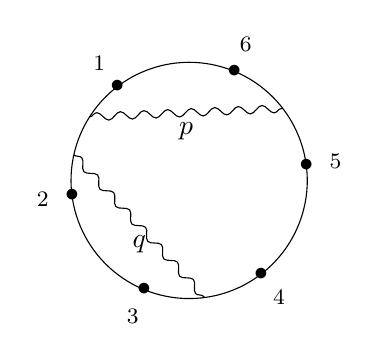
\begin{tikzpicture}[rotate=67.5,baseline=(current bounding box.east)] \begin{scope}
	\drawWLD{6}{1.5}
	\drawnumbers
	\drawlabeledprop{1}{-1}{5}{0}{$p$}
	\drawlabeledprop{1}{1}{3}{0}{$q$}
	\end{scope} \end{tikzpicture} \eas has a matrix \bas M_{\VP} = \begin{bmatrix} x_{p,1} &  x_{p,2} & 0 & 0 &x_{p,5} &x_{p,6} \\x_{q,1} &  x_{q,2} & x_{q,3} &  x_{q,4}& 0 & 0 \end{bmatrix}\; , \eas or, equivalently, can be written as \bas \cV = \{V_1 = \{1, 2, 5,6\} \; ; \; V_2 = \{1, 2, 3,4 \} \} \;.\eas The Grassmann Necklace of $\Sigma(\VP)$ is $GN(W) = \{ \{12\},\{23\}, \{35\}, \{45\}, \{51\}, \{61\} \}$. From \cite{casestudy}, we see that $\Sigma(\VP)$ shares a boundary with the positroid cells corresponding to \bas C(W_2) = \begin{bmatrix} *&  * & 0& 0 &0 &* \\ 0 &  * & *&  *& * & * \end{bmatrix}\eas and \bas C(W_3') = \begin{bmatrix} *&  * & *& 0 &0 &0 \\0 &  * & *&  *& * & * \end{bmatrix} \;. \eas Here the $*$ correspond not no-zero, independent real variables. In particular, the common boundary is parametrized by the matrix \bas M_{\cV}' = \begin{bmatrix} *&  * & 0& 0 &0 &0 \\0  &  * & *&  *& * & * \end{bmatrix}.\eas This common boundary is 5 dimensional, parameterized for instance by setting one of the stars in each row to be 1 and allowing the other entries to be free. From (\ref{eqn:rw_vanishes}), the vanishing set of $R(\VP)$ is exactly $L(\cV) \setminus \Sigma(\cV)$, where $L(\cV)$ is the geometric space parameterized by the matrix $M_{\VP}$. 

Let $\Sigma(\cV')$ be the positroid cell defined by the matrix $M_{\cV'}$. By construction $\Sigma(\cV')$ lies on the boundary of $\Sigma(\VP)$. We show that $\overline{\Sigma(\cV')}$ does not contain the vanishing loci of any of the factors of $R(\VP)$. The minors $\Delta_{13}$ and $\Delta_{15}$ are both non-vanising on $\Sigma(\cV')$, while $\Delta_{35}$ is uniformly zero. However, on $L(\cW)$, the nonvanishing of the minors $\Delta_{13}$ and $\Delta_{15}$ implies the nonvanishing of the minor $\Delta_{35}$. Since $\Delta_{35}$ vanishes on $\Sigma(\cV')$, $L(W)$ does not intersect this boundary and hence $R(\VP)$ does not vanish on $\Sigma(\cV')$.
\end{eg}

Below, we give a characterization of a class of variable valued matrices for which this type of boundary occurs. First, we extend the definitions of $\Prop(V)$ and $V_p$ for general variable valued matrices and not just those representing Wilson loop diagrams.

\begin{dfn}
Let $M_{\mathcal{V}}$ be a variable valued matrix as in definition \ref{dfn:variablevaluedmatrix}. Denote by $r$ a row of $M_{\cV}$, and $c$ a column of $M_{\cV}$. Then we write $\Cols(r)$ to be the columns where the row $r$ has non-zero entries. Similarly, write $\Rows(c)$ to be the rows where the column $c$ has non-zero entries. 
\end{dfn}

Note that if $M_{\mathcal{V}} = M_{\VP}$ the matrix associated to a Wilson loop diagram, the rows are the propagators and the columns are the vertices. Then $\Rows(c) = \Prop(c)$ and $\Cols(r) = V_r$.

We consider pairs of variable valued matrices defined as follows. Let $\Sigma(\cV)$ be a positroid cell of dimension $d$ in $\Gr(k,n)$, and $M_\cV$ be a variable valued matrix realizing $\Sigma(\cV)$ with a minimal number of independent variables. Let $V$ and $W$ be cyclic flats such that: \begin{enumerate} \item neither flat has full rank ($\rk (V), \; \rk(W) <k$), \item  The columns ($\Cols(V)$, $\Cols(W)$ and $\Cols(V \cup W)$) are cyclic intervals and \item one cyclc flat is not contained in the other (E.g. $W \not \subset V$) \end{enumerate}  Without loss of generality, suppose that the flat $V$ has non-zero entries in more rows outside of the rows of $W$ than vice versa: $|\Rows(V) \setminus \Rows(W)| \geq |\Rows(W) \setminus \Rows(V)|$. Then, construct the variable valued matrix $M_{\cV'}$ from $M_\cV$ by zeroing out the variable entries of $M_\cV|_{W}$ and inserting an equal number of non zero entries in $\Rows(V)$ and $\Cols(V\cup W)$ such that circuits in $V$ and $W$ are preserved. An example of this type of boundary pair is given in Example \ref{eg:strangeboundary} and explained in Example \ref{eg:strangeboundary2} below.


\begin{prop}\label{res:moving variables}
Let $M_\cV$ and $M_{\cV'}$ are variable valued matrices as above, and both have the same rank, then $M_{\cV'}$ defines a positroid, $\Sigma(\cV')$, that lies in the boundary of the positroid $\Sigma(\cV)$, the positroid defined by $M_\cV$. \end{prop}

\begin{proof} 
In this proof, we abuse notation, and use $M_\cV$ to indicate both the variable valued matrix, and its associated matroid.

We prove the theorem by showing that the Grassmann Necklace associated to $M_{\cV'}$, call it $GN(\cV')$ is different from the Grassmann Necklace defined by $M_{\cV}$, call it $GN(\cV)$, and that the basis set of $M_{\cV}$ contains the basis set of $M_{\cV'}$. In this way, we show that $\Sigma(\cV') \neq \Sigma(\cV)$, and that  $\Sigma(\cV')$ lies in the boundary of $\Sigma(\cV)$. 

First, we compare the Grassmann necklaces defining $\Sigma(\cV)$ and $\Sigma(\cV')$. We may read these directly off the matrices $M_{\cV}$ and $M_{\cV'}$. In particular, we with to show that that $GN(\cV) \neq GN(\cV')$. To see this, first note that $\rk(V)$ (resp. $\rk(W)$) $>0$. If this were not true, then whichever flat had rank $0$ would be contained in the other flat, which contradicts our hypothesis. Since $V \cup W$ is a cyclic interval (in both $M_\cV$ and $M_{\cV'}$), let $v$ denote the first element of $\Cols(V\cup W)$ in the $>_v$ ordering such that $\rk(v) >0$. Let $I_v$ and $I_v'$ be the Grassmann Necklace element starting at the column $v$ in $GN(\cV)$ and $GN(\cV')$ respectively. We have that $v \in I_v$ and $v \in I_v'$. 

Recally that $V$ and $W$ are both cyclic intervals and that $V \cup W$ is also cyclic interval. Without loss of generality, assume that $V$ preceeds $W$ in the $>_v$ ordering. Write $I_v = \{v = v_1, \ldots, v_r, w_1, \ldots w_s, u_1, \ldots u_t\}$, where $v_i \in V$, $w_i \in W$ and $u_i \not \in (V \cup W)$. From this, we can see that $\rk(V) = r$ and $\rk(V\cup W) = r+s$. Furthermore, since $W$ is not a subset of $V$, we know that $s > 0$. 

Suppose, for contradiction, we have that $GN(\cV) = GN(\cV)$. Then we would have $I_v = I'_v$. But this would imply that $\rk(V \cup W)$ in $C'$ is $r+ s$. However, by construction, in $C'$, $\rk(V) = \rk(V\cup W)$, i.e. $r = r+s$ which contradicts the fact that $s > 0$. 

\begin{comment}
 inote that some vertex of $V$ (resp. $W$)  appears at least once in $GN(C)$. To see this, note that any element that does not ever appear in $GN(C)$ has rank $0$. Since neither $V$ nor $W$ has rank $0$, they must each contain at least one element that appears in $GN(C)$. Therefore, we know that there exists some $I_j \in GN(C)$ such that $I_j \cap W \neq \emptyset$. Fix such a $j$ and let $a \in  I_j \cap W$ be an element of $W$ that is in said $I_j$. Let $I'_j$ be the correposponding element of $GN(C')$. We claim that $I_j \neq I_j'$. That is, the $j^{th}$ minor in $GN(C')$ is not the same as the $j^{th}$ minor of $GN(C)$. This shows that $M(C)$ and $M(C')$ define two different positroid cells. Then it remains to show that the the basis set $\cB$ of $M(C)$ contains the basis set $\cB'$ of $M(C')$. 

\emph{Proof of claim:}Suppose, for contractiction, $I_j = I'_j$. Write $I_j = v_1 \ldots v_k$ with $v_i <_j v_{i+1}$. By definition fo the Grassmann Necklace, $a$ is the first column in the $>_j$ ordering of the columns of $C$ that is not contained in the flat defined by previous elements of $I_j$: $\textrm{cl}(\{v_i | v_i <_j a \})$ in $M(C)$. In $C'$, the non-zero entries in the column $a$ lie in the rows where $V$ has non-zero entries: $\Rows(a) \subset \Rows(V)$. Since $a \in I'_j$, the flat $V \cup W$ in $M(C')$ is not contained in the the flat defined by the previous elements of $I'_j$: $V \cup W \not \subset \textrm{cl}(\{v_i | v_i <_j a )$ in $M(C')$. Since $\Rows(V \cup W)$ in $C'$ is the same as $\Rows(V)$ in $C$, the flat defined by $V$ in $M(C)$ is is not contained in the the flat defined by the previous elements of $I_j$: $V\not \subset \textrm{cl}(\{v_i | v_i <_j a ) \}$ in $M(C)$. \todo{is $U$ uniquely defined?} Let $U \subset I_j$ be the smallest subset of $I_j$ that is needed to ensure that $V \subset \textrm{cl}(\{v_i | v_i <_j a \} \cup U)$ in $M(C)$. Note that $a$ preceeds all elements of $U$, by construction s $a \leq_j u$ for all $u \in U$ in $M(C)$. However, also by construction, $a \in U$ in $M(C')$. Therefore, there must be some $b \in U$ that is in $M(C)$ but not in $M(C')$, thus violating $I_j = I'_j$.
\end{comment} 

To see that basis set $\cB$ of $M_\cV$ contains the basis set $\cB'$ of $M_{\cV'}$, note that any $B \in \cB$ that that does not intersect $V \cup W$ is also a basis set of $\cB'$ and vice versa. Let $B' \in \cB'$ be a basis set of $M_{\cV'}$ intersecting $V\cup W$. Partition $B'$ into two sets, those elements in $V \cup W$  and those not: $B' = B'_1 \cup B'_2$ with $B'_1 \subset V \cup W$ and $B'_2 \cap (V \cup W) = \emptyset$. If $B'$ were not a basis set of $M(\cV)$ ($B' \not \in \cB$), then $B'_1$ contains a circuit in $C$. But this would imply that a set of columns that formed a circuit in $M_{\cV}|_V$ or $M_\cV|_W$ became an independent set in $M_{\cV'}$ which violates the construction.
\end{proof}

\begin{eg}\label{eg:strangeboundary2}
Continuing with Example \ref{eg:strangeboundary2}, if $\cV = \{V_p = \{1, 2, 5, 6\}, V_q = \{1, 2, 3, 4\}\}$, we may write $C(V_1) = M_\cV$. Let $W = \{ 3, 4\}$, and $V = \{5, 6\}$ are cyclic flats that satisfy the conditions of the proposition. Then, up to permuations of the rows, there is only one choice for $M_{\cV'}$: \bas M_{\cV'} = \begin{bmatrix} *&  * & 0& 0 &0 &0 \\ *  &  * & *&  *& * & * \end{bmatrix}. \eas Not that while this is not the same matrix as $M_{\cV'}$ in Example \ref{eg:strangeboundary}, these two matrices do represent the same matriod. (This can be seen by comparing basis sets.)
\end{eg}

In order to see that, given a minimal parametrization $M_{\cV'}$, the product of the Grassmann Necklace minors, $R(\cV)$\todo{introduce this notation} doesn't vanishon the boundary we need to apply consider the minors $I_v$ and $I'_v$ defined in Proposition \ref{res:moving variables}. The follow proof follows the logic of  Example \ref{eg:strangeboundary}.

\begin{thm}
Given a matrix $M_{\cV}$ and $M_{\cV'}$ as above, the polynomial $R(\cV)$ does not vanish on $\Sigma(\cV')$. 
\end{thm} \todo{Cam: check this for correctness}

\begin{proof}
Consider the Grassmann Necklace elements $I_v$ and $I'_v$ as above, elements of the Grassmann Necklaces for $GN(\cV)$ and $GN(\cV')$ respectively. Since $\Sigma(\cV')$ is a boundary cell of $\Sigma(\cV)$, the basis set of $M(\cV')$ is contained in the basis set of $M(\cV)$. Namely, $I'_v$ is a basis set for both $M(\cV)$ and $M_(\cV')$, but $I_v$ is one only for $M(\cV)$. Then select two elements, $a = I'_v \setminus I_v$ and $b = I_v \setminus I'_v$. Note that the set $I'_v$ must contain elements not in the cyclic flat $V \cup W$, otherwise, $I'_v$ would not have full rank in $M(\cV')$. Therefore, chose $a$ to not be in $V \cup W$. Then, by the basis exchange theorem, there is a basis set $B = (I_v \setminus b)\cup a$, and the non-vanishing of any two of the minors $\{\Delta_{I_v}, \Delta_{I'_v}, \Delta_{B}\}$ in $M_\cV$ implies the non-vanishing of the third. However, in $M_{\cV'}$, $\Delta_{I_v}$ is uniformly zero. Therefore, $L(\cV)$ does not contain the positroid cell $\Sigma(\cV')$.

By display \eqref{eqn:rw_vanishes}, we have that $R(\cV)$ vanishes on $L(\cV) \setminus \Sigma(\cV)$. Therefore, $R(\cV)$ does not vanish on $\Sigma(\cV')$. 
\end{proof}

\begin{rmk}
In particular, not that the construction $M_{\cV'}$ need not have the minimal number of parameters to represent $\Sigma(\cV')$. In particular, we have that  \bas |\bigcup_{V \in \cV}V| = 6 \quad \textrm{ while } \max_{V \in  \cV} (|V|) + |\mathcal{V}| +1 = 5 + 2 +1 = 8 \;.\eas Therefore, setting $\cV = \mathcal{T}$, we see that the third equivalence of Theorem \ref{ref:minimalrep} doesn't hold, and thus $M_{\cV'}$ is not a minimal representation. In fact, there is a $Gl(k)$ transformation taking $M_{\cV'}$ to $\D_1$: \bas \begin{bmatrix}1 & 0  \\ -\frac{x_{q_1}}{x_{p_1}} & 1 \end{bmatrix}  \begin{bmatrix} x_{p,1}&  x_{p,2} & 0& 0 &0 &0 \\x_{q,1}  &  x_{q,2} & x_{q,3}&  x_{q,4}& x_{q,5} & x_{q,6} \end{bmatrix} =  \begin{bmatrix} x_{p,1}&  x_{p,2} & 0& 0 &0 &0 \\0  &  x_{q,2} -\frac{x_{q_1}x_{p_2}}{x_{p_1}} & x_{q,3}&  x_{q,4}& x_{q,5} & x_{q,6} \end{bmatrix} \eas \end{rmk}


\begin{rmk}
The requirement that $V$ and $W$ are cyclic intervals may seem arbitrary until one considers that all flacets of a matroid are cyclic intervals if and only if the matroid is a positroid, and that all flacets are cyclic intervals. In some moral sense, the algorithm prescribed in Proposition \ref{res:moving vairables} aims to combine two flacets into a larger flacets in order to define a new positroid cell. 
\end{rmk}

In the particular case of Wilson loop diagrams ($W = (\cP, [n])$), recall from Lemma 2.28 of \cite{wilsonloops} that all cyclic flats can be represented as a propagator flat, $F(P)$, and that be Lemma 3.35 of the same, any propagator flat that is a cyclic flat has rank equal to the number of propagators in the set defining it. Therefore, the boundaries of the sort considered above occur when there are two propagators flats $F(P)$ and $F(Q)$ such that \begin{enumerate} \item Neither $P$ nor $Q$ are the full propagators set, $\cP$. \item The sets $F(P)$, $F(Q)$ and $F(P) \cup F(Q)$ form cylic intervals in $[n]$, \item On propagators set is not contained in the other. \end{enumerate} It is easy to check that these conditions are met in the Wilson loop diagram $W$ in Examaple \ref{eg:strangeboundary}.

We are now ready to prove the main result of this section: that the singularities of $I(\VP)$ that lie on codimension $1$ boundaries of $\Sigma(\VP)$ all cancel in the tree amplitude. Before we begin, we recall a few facts about the polynomial $R(\VP)$. As a motivating example, we consider the diagram \ba W =   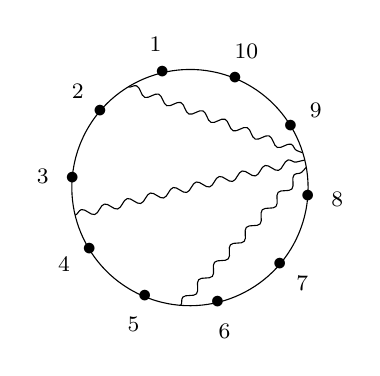
\begin{tikzpicture}[rotate=67.5,baseline=(current bounding box.east)]
	\begin{scope}
	\drawWLD{10}{1.5}
	\drawnumbers
	\drawprop{1}{0}{8}{1}
	\drawprop{3}{0}{8}{0}
        \drawprop{5}{0}{8}{-1}
		\end{scope}
	\end{tikzpicture} \label{eq:relevantexample}\ea with the associated matrix \bas  M_{\VP}  = \begin{bmatrix}  x_{p,1} & x_{p,2} &0 & 0 & 0 & 0& 0 & x_{p,8} & x_{p,9} & 0 \\ 0 &  0 & x_{r,3} & x_{r,4} & 0  & 0  & 0 & x_{r,8} & x_{r,9} & 0  \\  0 & 0 & 0 &0 &x_{s, 5}  &x_{s,6}& 0  & x_{s,8} & x_{s, 9} & 0 \end{bmatrix} \;.\eas 

Every codimension one pole of an admissible Wilson loop diagram is a factor of the polynomial $R(\VP)$ appearing in the denominator of the associated integrand. By Definition \ref{dfn:I(W)}, the primitive factors of $R(\VP)$ either either have degree one or two, corresponding to $1 \times 1$ or $2 \times 2$ minors of $M_{\VP}$. Infact, by this definiton, the degree one factors of $R(\VP)$ are of the form  $x_{q_1, e+1}$ or $x_{q_s, e}$. Setting these factors to $0$ correspons to changing the support of either the first or the last propagators supported on the edge $e$ such that the first propagator is no longer supported by the vertex $e +1$ (i.e.  $x_{q_1, e+1} = 0 $) or the last propagator is not supported on the vertex $e$, (i.e. $x_{q_1, e} = 0$). For instance, for $W$ as in \eqref{eq:relevantexample}, we depict this diagramatically, for $e = 8$ as \bas   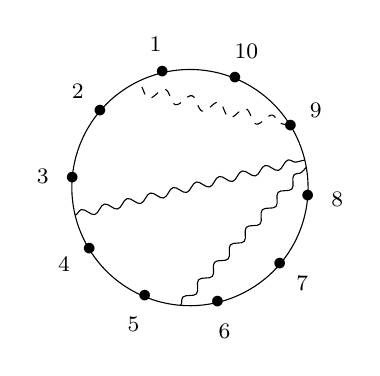
\begin{tikzpicture}[rotate=67.5,baseline=(current bounding box.east)]
	\begin{scope}
	\drawWLD{10}{1.5}
	\drawnumbers
	\boundaryprop{1}{0}{9}{propagator, dashed}
	\drawprop{3}{0}{8}{0}
        \drawprop{5}{0}{8}{-1}
		\end{scope}
	\end{tikzpicture} \text{ or } 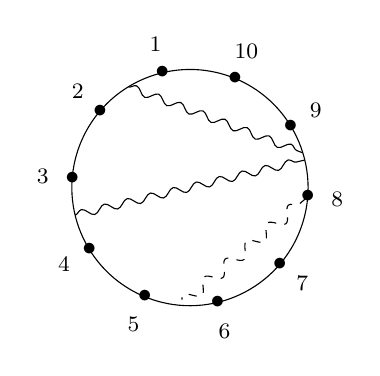
\begin{tikzpicture}[rotate=67.5,baseline=(current bounding box.east)]
	\begin{scope}
	\drawWLD{10}{1.5}
	\drawnumbers
	\drawprop{1}{0}{8}{1}
	\drawprop{3}{0}{8}{0}
        \boundaryprop{5}{0}{8}{propagator, dashed}
		\end{scope}
	\end{tikzpicture} \;.\eas Note that unless there is exactly one propagator adjascent on an edge, there is at most ever one variable corresponding to that edge that is a factor of $R(\VP)$. 

Similarly, the degree two factors corresponds to setting two pairs of variables, ($x_{q_i, e} , x_{q_i e+1}$) and ($x_{q_{i+1}, e} , x_{q_{i+1}, e+1}$), precicely those supporting adjasacent propagators on an edge, as scalar multiples of each other. Diagramatically, we depict this as  we draw this by making two adjascent propagators meet on the common edge. Again, from display \eqref{eq:relevantexample}, with $e = 8$, \bas   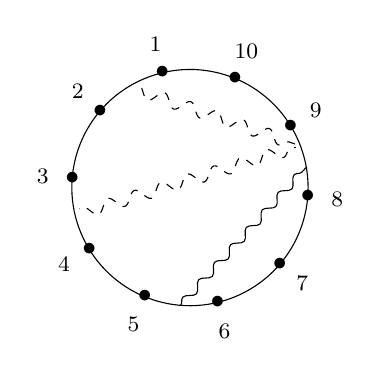
\begin{tikzpicture}[rotate=67.5,baseline=(current bounding box.east)]
	\begin{scope}
	\drawWLD{10}{1.5}
	\drawnumbers
	\modifiedprop{1}{0}{8}{2}{propagator, dashed}
	\modifiedprop{3}{0}{8}{2}{propagator, dashed}
        \drawprop{5}{0}{8}{-1}
		\end{scope}
	\end{tikzpicture} \;.\eas. Note that there is never any factor of $R(\VP)$ that involves two non-adjascent propagators.   

\begin{thm} \label{res:deg1polescancel}
All the codimension 1 poles of admissible Wilson loop diagrams cancel.
\end{thm}

\begin{proof}

We first consider all the possible degree 1 factors of $R(\VP)$. Write $W = (\cP, [n])$ with $p= (i,j)  \in \cP$. Suppose $j > i+2$ (i.e. if $V_p$ does not consist of $4$ cyclically consecutive vertices) and, wihtout loss of generality, assume $x_{p, i}$ is a factor of $R(\VP)$. Then if $q = (i+1, j) \not \in \cP$ the we may define another diagram $W' = ((\cP \setminus p) \cup q, [n])$ such that $\lim_{x_{p, i} \rightarrow 0} I(\VP) = -\lim_{x_{q, i+2} \rightarrow 0} I(W')$, where the negative sign comes from the evaluation of $\delta^{4k|4k}$ (see Lemma \ref{lem:movingpropnegative}). For more details on the minus signs, see \cite{casestudy, HeslopSteward, correlahedron}. By the arguments of \cite{basisshapeloci}, we see that this parametrizes a co-dimension 1 boundary of $\Sigma(\VP)$. It is easy to check that $W'$ satisfies both non-crossing (because $W$ satisfies non-crossing) and the density (because $q \not \in \cP$, and $W$ satisfies density) conditions for admissibility. Therefore $W'$ is admissible. 

If $q = (i+1, j) \in \cP$, then, in the matrix $\lim_{x_{p, i} \rightarrow 0}M_{\VP}$, the row corresponding to the propagator $p$ now has 3 non-zero entries (corresponding to the columns $\{i+1, j, j+1\}$) and the row corresponding to $q$ has $4$ non-zero entries (corresponding to the columns $\{i+1, i+2, j, j+1\}$). That is, we have $2$ rows with non-zero entries in $4$ columns. Therefore, by Theorem \ref{res:minimalrep}, we see that this parametrizes a co-dimension 2 boundary of $\Sigma(\VP)$. Therefore, we do not consider these poles in this argument. 

It remains to consider the degree one factors of $R(\VP)$ contributed by propagators of the form $p = (i, i+2)$. If $x_{p, i+1}$ or $x_{p, i+2}$ is a factor of $R(\VP)$, then consider the propatator $q = (i-1, i+2)$ or $q = (i, i+3)$ respectively. If $q \not \in \cP$, then the diagram $W' = ((\cP \setminus p)\cup q, [n])$ is admissible, and the argument proceeds as above, using Lemma \ref{lem:movingpropnegative}. If $q \in \cP$, then by the arguments above, by Theorem \ref{res:minimalrep}, we see that the matrix $\lim_{x_{p, i+1} \to 0} M_{\VP}$ (resp. $\lim_{x_{p, i+1} \to 0} M_{\VP}$) parametrizes a co-dimension 2 boundary of $\Sigma(\VP)$. Therefore we do not consider this case. If $x_{p, i}$ or $x_{p, i+3}$ is a factor of $R(\VP)$, consider $q = (i+1, i+3)$ and $q = (i-1, i+1)$ respectively. By the non-crossing condition, $p$ and $q$ cannot simultaneously exist in $W$. If $W$ does not contain another propagator of the form $(i+2, k)$ or $(i, k)$ respectively, we may define an admissible diagram $W' = ((\cP \setminus p)\cup q, [n])$ (otherwise, $q$ would cross the existing propagator $(i+2, k)$ or $(i, k)$).  In this case, $\lim_{x_{p, i} \rightarrow 0} I(\VP) = -\lim_{x_{q, i+4} \rightarrow 0} I(W')$ where the negative sign again comes from Lemma \ref{lem:movingpropnegative}.

It remains to check the case when $x_{p, i}$ (resp. $x_{p, i+3}$) is a factor of $R(\VP)$ and there exists a propagator $(i+2, k)$ (resp. $(i, k)$) in $W$. In this case, the simple pole formed by taking the limit as $x_{p, i}$ (resp. $x_{p, i+3}$) goes to zero cancels with a pole coming from degree 2 factors contributed by other diagrams. Therefore, we return to this during the discussion of $2 \times 2$ minors. 

Next, we consider the degree 2 factors of $R(\VP)$. In order for such a factor to exist, there must be some edge of $W$, call it $i$, that has at least two propagators ending on it, say $p = (i, j)$ and $q = (i, k)$. Suppose $k > j+1$, that is, the other endpoints of $p$ and $q$ are not on adjascent edges. If $r = (j,k) \not \in \cP$, consider two other diagrams $W' = ((\cP \setminus p) \cup r, [n])$ and $W'' = ((\cP \setminus q) \cup r, [n])$. Since $k> j+1$ and $r \not \in \cP$, both $W'$ and $W''$ both satisfy density. Furthermore, since $W$ is admssible, and $p$ and $q$ are adjascent on the edge $i$, there does not exist a propagator $(i, m)$ with $j < m <k$, that is, that has one endpoint on the $i^{th}$ edge, and the other between the endpoints of $p$ and $q$. Therefore, $W'$ and $W''$ satisfy non-crossing. I.e, they are both admissible. Note that the diagrams $W$, $W'$ and $W''$ are in the configuration layed out in display \eqref{eq:wideV}. By Theorem \ref{res:Rado}, we see that the reparametrization performed in Lemma \ref{res:Vdiagcancel} means that $\lim_{(x_{p,i}x_{q,i+1} -x_{p,i+1}x_{q,i})\rightarrow 0} M_{\VP}$  parameterized a codimension 1 subspace of $\overline{\Sigma(\VP)}$. By Proposition \ref{res:vanishonbdny}, this is lies in a codimension 1 boundary of $\Sigma(\VP)$. Accoring to Lemma \ref{res:Vdiagcancel}, after appropriate changes of parametrizations, one may write \bas \lim_{(x_{r,k}x_{q,k+1} -x_{r,k+1}x_{q,k})\rightarrow 0}I(W') +  \lim_{(x_{p,i}x_{q,i+1} -x_{p,i+1}x_{q,i})\rightarrow 0} I(\VP) + \lim_{(x_{p,j}x_{r,j+1} -x_{p,j+1}x_{r,j})\rightarrow 0}I(W'') = 0 \; .\eas 
\begin{comment}
That is, the limits represented by the following diagrams, paramterize the same codimension 1 subspace in the intersection $\Sigma(\VP) \cap \Sigma(W') \cap \Sigma(W'')$.    \bas 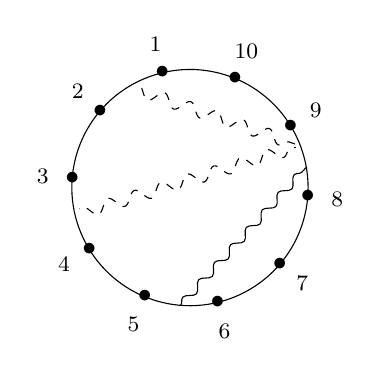
\begin{tikzpicture}[rotate=67.5,baseline=(current bounding box.east)]
	\begin{scope}
	\drawWLD{10}{1.5}
	\drawnumbers
	\modifiedprop{1}{0}{8}{2}{propagator, dashed}
	\modifiedprop{3}{0}{8}{2}{propagator, dashed}
        \drawprop{5}{0}{8}{-1}
		\end{scope}
	\end{tikzpicture} \leftrightarrow 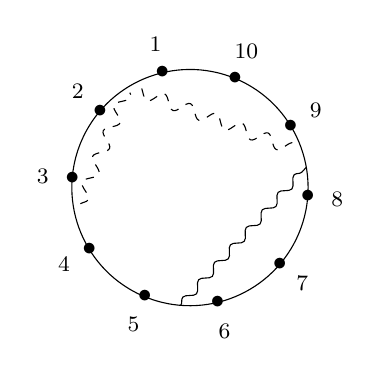
\begin{tikzpicture}[rotate=67.5,baseline=(current bounding box.east)]
	\begin{scope}
	\drawWLD{10}{1.5}
	\drawnumbers
	\modifiedprop{1}{0}{8}{1}{propagator, dashed}
	\modifiedprop{1}{0}{3}{0}{propagator, dashed}
        \drawprop{5}{0}{8}{-1}
		\end{scope}
	\end{tikzpicture} \leftrightarrow 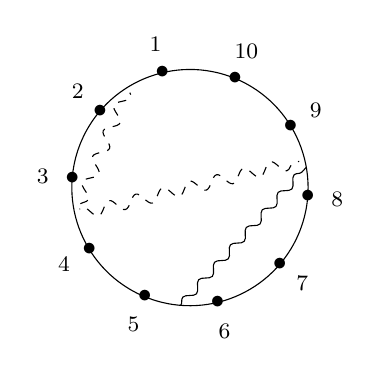
\begin{tikzpicture}[rotate=67.5,baseline=(current bounding box.east)]
	\begin{scope}
	\drawWLD{10}{1.5}
	\drawnumbers
	\modifiedprop{1}{0}{3}{0}{propagator, dashed}
	\modifiedprop{3}{0}{8}{0}{propagator, dashed}
        \drawprop{5}{0}{8}{-1}
		\end{scope}
	\end{tikzpicture}\eas \end{comment}
In otherwords, these three codimension 1 boundaries cancel in the sum of integrals tha make up the amplitude.

If $k > j+1$ but the propagator $r =  (j,k) \in \cP$, we claim that setting any of the minors $(x_{p,i}x_{q,i+1} -x_{p,i+1}x_{q,i})$, $(x_{p,j}x_{r,j+1} -x_{p,j+1}x_{r,j})$ or $(x_{r,k}x_{q,k+1} -x_{r,k+1}x_{q,k})$ to zero parametrized a space of codimension greater than 1. Without loss of generality, consider the case where $(x_{p,i}x_{q,i+1} -x_{p,i+1}x_{q,i}) = 0$. Then by adding a scalar multiple of the row corresponding to column $p$ to the row corresponding to the column $q$, one may reparametrize $M_{\VP}$ such that $V_{q'} = V_r = \{j, j+1, k, k+1\}$. Thus, we have 2 propagators supported on $4$ vertices, and by Theorem \ref{res:minimalrep}, this is not a minimal representation of $M_{\VP}$. In particular, one may perform a $GL(k)$ transformation on $M_{\VP}$ that acts as the identity on the rows corresponding to all rows except $q$ and $r$. Under this transformation, the rows corresponding to the propagators $q$ and $r$ have non-zero entries in columns $V_{q''} = \{j, k, k+1\}$ and $V_{r''} = \{j+1, k , k+1\}$ respectively. Thus after 2 applications of $GL(k)$ transforamations, we have reduced the number of non-zero entries of $M_{\VP}$ by 2, showing that the surface where $(x_{p,i}x_{q,i+1} -x_{p,i+1}x_{q,i}) = 0$ has co-dimension of at least 2 in $\Sigma(\VP)$. \todo{still don't like this argument. Cleaner ideas?}

It remains to check the case where $k = j+1$, i.e. $W$ contains a pair of propagotors configured as below: \bas 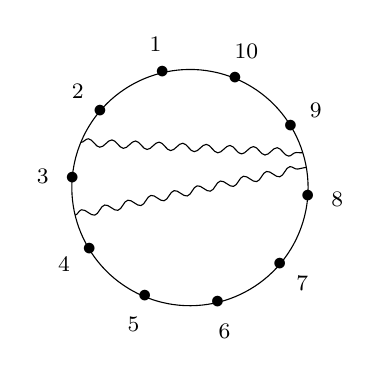
\begin{tikzpicture}[rotate=67.5,baseline=(current bounding box.east)]
	\begin{scope}
	\drawWLD{10}{1.5}
	\drawnumbers
	\drawprop{3}{0}{8}{-1}
	\drawprop{2}{0}{8}{1}
		\end{scope}
	\end{tikzpicture} \eas

Consider the diagrams $W' = ((\cP \setminus p) \cup r = (j, j+2), [n])$ and $W'' = ((\cP \setminus p) \cup s = (k-2, k), [n])$. Since the edge $r \not \in \cP$ (it would cross $q$ if it were), and $s \not \in \cP$ (it would cross $p$ if it were), we see that $W'$ and $W''$ satisfy both the non-crossing and density conditions, and thus are admissible. Furthermore, $W$, $W'$ and $W''$ are in the configurations layed out in display \eqref{eq:narrowV}.

We see from Lemma \ref{res:narrowVcancel} that pole defined by the limit of sending $(x_{p,i}x_{q,i+1} -x_{p,i+1}x_{q,i})$ to $0$ cancels with degree 1 poles in the diagrams in $W'$ and $W''$ under the correct parametrizations: \bas \lim_{(x_{p,i}x_{q,i+1} -x_{p,i+1}x_{q,i}) \rightarrow 0}I(\VP) + \lim_{x_{r, k-2}\rightarrow 0}I(W') + \lim_{x_{s, j+3}\rightarrow 0}I(W'') =0 \;.\eas That is, the limits represented by the following diagrams, paramterize the same codimension 1 subspace in the intersection $\Sigma(\VP) \cap \Sigma(W') \cap \Sigma(W'')$.
\begin{comment}
 \bas 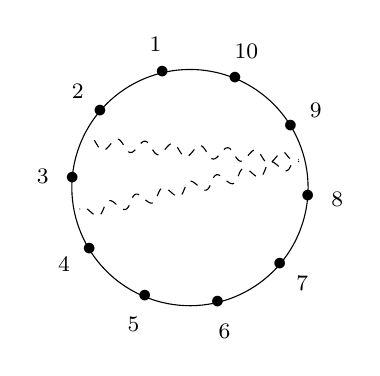
\begin{tikzpicture}[rotate=67.5,baseline=(current bounding box.east)]
	\begin{scope}
	\drawWLD{10}{1.5}
	\drawnumbers
        \modifiedprop{3}{0}{8}{0}{propagator, dashed}
	\modifiedprop{2}{0}{8}{0}{propagator, dashed}
	\end{scope}
	\end{tikzpicture} \leftrightarrow 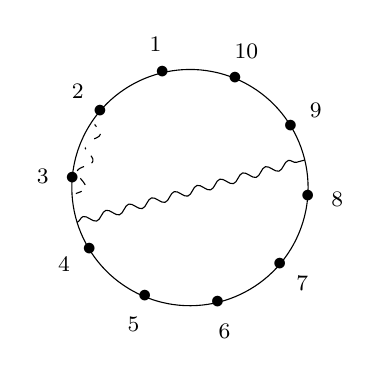
\begin{tikzpicture}[rotate=67.5,baseline=(current bounding box.east)]
	\begin{scope}
	\drawWLD{10}{1.5}
	\drawnumbers
        \drawprop{3}{1}{8}{0}
	\boundaryprop{3}{-1}{2}{propagator, dashed}
	\end{scope}
	\end{tikzpicture} \leftrightarrow 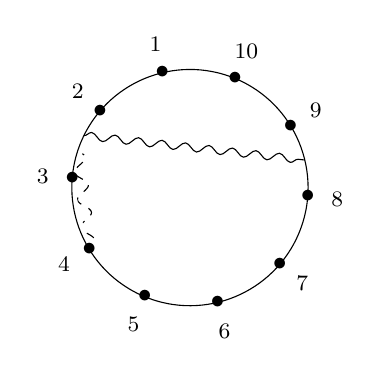
\begin{tikzpicture}[rotate=67.5,baseline=(current bounding box.east)]
	\begin{scope}
	\drawWLD{10}{1.5}
	\drawnumbers
        \drawprop{2}{-1}{8}{0}
	\boundaryprop{2}{1}{4}{propagator, dashed}
	\end{scope}
	\end{tikzpicture}\eas
\end{comment}
Note that the degree one terms of $R(\VP)$ involved in this calculation are exactly the degree one factors whose cancelation was put off until discussion of the degree two terms.
\end{proof}


\begin{rmk}
We remark that this cancelation is exact only in the space parametrized by matrices of the form $M(\VP)$, as a subspace of $\Gr(k,n)$ and not in the space parametrized by matrices of the form $M(\YP)$, as a subspace of $\Grall(k,n+1)$. In \cite{HeslopStewart,non-orientability}, the authors explicitly show that cancelations of this form do not hold in the larger space because of orientation issues.
\end{rmk}

\begin{appendices} 
\section{Graveyard of Technical Lemmas \ref{sec:appendix}}
In this section, we present some calculations to aid in the understanding of the cancelation of spurious poles. Many of the results here can be found in \cite{casestudy, correlahedron, HeslopStewart}. However, they are presented here for completeness.

Recall from definition \ref{dfn:I(W)} that \bas \cI(\VP) (\cZ_*)  = \int_{(\RP^4)^k} \frac{\prod_{p \in \cP} \prod_{v \in V_p} dx_{p, v}}{R(\VP)} \delta^{4k|4k}(x_*(W) \cdot \cZ_*) \eas where, for $X$ a $k \times n+4$ matrix, \bas \delta^{4k|4k}(X) = \prod_{b =1}^k (X_{b, 4+b})^4\delta^4((X_{b,1},X_{b,2},X_{b,3},X_{b,4}))  \;.\eas Write $\cZ_*^i$ to indicate the $i^{th}$ column of $\cZ_*$ and $\cZ_*^\mu$ to indicate the matrix formed by taking the first 4 columns of $\cZ_*$. Then evaluating the integral $I(\VP)$ corresponds to localizing the expression \bas \frac{\prod_{b = 1}^k (Y_b \cdot \cZ_*^b)^4}{R(\VP)}\eas at the solution to $x_*(W) \cdot \cZ_*^\mu = 0$. By Cramer's rule, we see that this localization evaluates \ba x_{p, 0} &= \det(Z_i^\mu, Z_{i+1}^\mu, Z_{j}^\mu, Z_{j+1}^\mu ) \\ x_{p, i} = \det(Z_0^\mu, Z_{i+1}^\mu, Z_{j}^\mu, Z_{j+1}^\mu ) \; &; \; x_{p, i+1} = \det( Z_{i}^\mu, Z_0^\mu, Z_{j}^\mu, Z_{j+1}^\mu ) \; \text{ etc.} \label{eq:matrixvalues}\ea That is, the entry $x_{p, m}$ evaluates to the minor of $\cZ_*^\mu$ indicated by the rows in $V_p$, with the $m^{th}$ row replaced by $Z_0^\mu$.

\begin{lem} \label{lem:movingpropnegative}
For two propagators $p = (i, j)$ and $q = (i, j+1)$, after localization $x_{p, j} = -x_{q, j+2}$
\end{lem} 

\begin{proof}
By the above arguments, note that $x_{p, j} = \det(Z_i^\mu, Z_{i+1}^\mu, Z_{0}^\mu, Z_{j+1}^\mu )$ while $x_{q, j+2} = \det(Z_i^\mu, Z_{i+1}^\mu, Z_{j+1}^\mu , Z_{0}^\mu )$. Thus these two values are negatives.
\end{proof}

Sometimes, it is necessary to perform changes of variables in order to perform the cancellation of variables. For ease of calculation, we introduce a simplifying change of variables:
\begin{lem}\label{lem:simplifyR(W)}
When two propagators $p = (i, j)$ and $q = (i, k)$ are \hlfix{adjacent }{note, we need to keep the order in mind for this reparameter} on an of $W$, then there is a reparametrization under which one can replace the factor $x_{p, i}(x_{p, i}x_{q, i+1} - x_{p, i+1}x_{q, i})x_{q, i+1}$ in $R(\VP)$ with the product of 4 terms: $xyzw$.
\end{lem}

\begin{proof}
We restrict our attention to the relavant $2 \times 2$ minor of $x_*(W)$, $ \begin{bmatrix} x_{p, i} & x_{p, i+1} \\ x_{q, i} & x_{q, i+1} \end{bmatrix} $,  which we can reparametrize as $ \begin{bmatrix} x & y \\ xz & zy + w \end{bmatrix} $. Then we have that \bas x_{p, i} = x \quad ; \quad  x_{p, i+1} = y \quad ; \quad x_{q, i} = xz\quad  ;\quad x_{q, i+1}  = zy + w \; . \eas Furthermore, \bas dx_{p, i} = dx  \quad ; \quad  d x_{p, i+1} = dy \quad ; \quad dx_{q, i} = x dz + z dx \quad ; \quad d x_{q, i+1} = ydz + z dy + dw \;.\eas Therefore, under these changes of variables, we see that \bas \frac{dx_{p, i}\;dx_{p, i+1}\;dx_{q, i}\;dx_{q, i+1}}{x_{p, i+1}(x_{p, i}x_{q, i+1} - x_{q, i}x_{p, i+1} ) x_{q, i}}  = \frac{ dx\;dy\;x dz\; dw}{y (xyz + xw - xyz)xz}\eas which simplifies to the desired result.
\end{proof}

In future, we use whichever parametrization of the $2 \times 2$ minors is convenient. The need for a change of variables comes up in two cases. The first case involves the cancelation of the $2 \times 2$ minors in following three propagator confgurations: \bml \textrm{Config 1} = 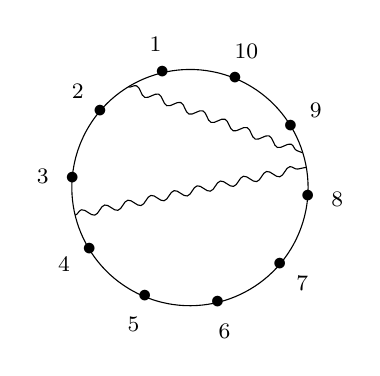
\begin{tikzpicture}[rotate=67.5,baseline=(current bounding box.east)]
	 \begin{scope}
	\drawWLD{10}{1.5}
	\drawnumbers
	\drawprop{1}{0}{8}{1}
	\drawprop{3}{0}{8}{-1}
		\end{scope}
	\end{tikzpicture} \quad ; \quad \textrm{Config 2} = 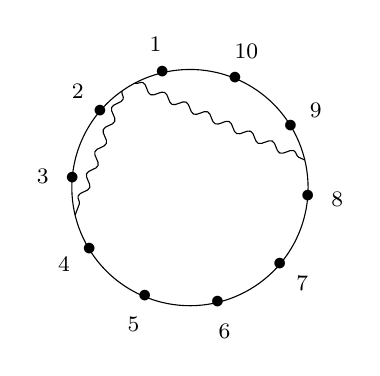
\begin{tikzpicture}[rotate=67.5,baseline=(current bounding box.east)]
	\begin{scope}
	\drawWLD{10}{1.5}
	\drawnumbers
	\drawprop{1}{-1}{8}{0}
	\drawprop{1}{1}{3}{0}
		\end{scope}
	\end{tikzpicture} \\ \textrm{Config 3} = 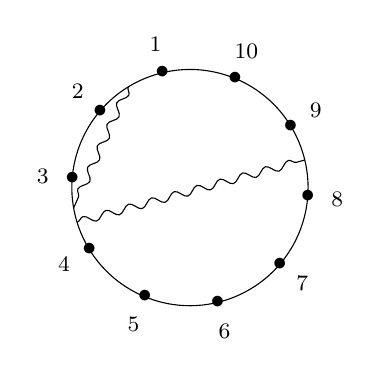
\begin{tikzpicture}[rotate=67.5,baseline=(current bounding box.east)]
	\begin{scope}
	\drawWLD{10}{1.5}
	\drawnumbers
	\drawprop{1}{0}{3}{-1}
	\drawprop{3}{1}{8}{0}
		\end{scope}
	\end{tikzpicture} \label{eq:wideV}\eml

\begin{lem}\label{res:Vdiagcancel}
Let $W_1$, $W_2$ and $W_3$ be admissible Wilson loop diagrams that are identical except for the fact that the diagram $W_i$ cotains the pair of adjascent propagators shown in $\textrm{Config i}$ above. Then 
\bas \sum_{i = 1}^3 \lim_{\textrm{degree 2 factor of } R(W_i) \rightarrow 0} I(W_i) = 0\;.\eas \end{lem}

This proof is also given in \cite{HeslopStewart, casestudy} but is included here for completeness.
\begin{proof}
Without loss of generality, write $(x_*(W_i))$ with the pertinent propagators represented in the first two rows. Then the matrices $x_*(W_i)$ are identical except for the first two rows. Since the propagators are adjacent, by Lemma \ref{lem:simplifyR(W)} we may write the first two rows as \bas x_*(W_1) = \begin{bmatrix}1 & \ldots & a &b &\ldots & 0 & 0 & \ldots & c & d   \ldots\\  1 & \dots &  ae &be + f  & \ldots &g & h & \ldots &0 &0  \ldots   \end{bmatrix}  \\ x_*(W_2) = \begin{bmatrix}1 & \ldots & a' & b' &\ldots & c' & d' & \ldots & 0 & 0   \ldots\\  1 & \dots &  0 & 0  & \ldots &c'e' & d' e' + f' & \ldots &g' &h'  \ldots   \end{bmatrix} \\x_*(W_3) = \begin{bmatrix}1 & \ldots & 0 &0 &\ldots & a'' & b'' & \ldots & c'' & c''   \ldots\\  1 & \dots &  e'' & f''  & \ldots &0 & 0 & \ldots &c''g'' & d'' g'' + h'' \ldots   \end{bmatrix}\;.\eas We multiple the first two rows of $x_*(W_2)$ and $x_*(W_3)$ by elements of $GL(2)$, leaving the rest of the rows unchanged. Namely, consider the products: \bas \begin{bmatrix} \frac{- e'}{1-e'} & \frac{1}{1-e'} \\ 1 & 0  \end{bmatrix} x_*(W_2) = \begin{bmatrix}  1 & \dots & \frac{-e' a'}{1- e'}  & \frac{-e' b'}{1- e'}  & \ldots &0 & \frac{ f'}{1-e'} & \ldots &\frac{g'}{1-e'} &\frac{h'}{1-e'}  \ldots  \\ 1 & \ldots & a' & b' &\ldots & c' & d' & \ldots & 0 & 0   \ldots \end{bmatrix}  \\ \begin{bmatrix}  \frac{1}{1-c''} & \frac{-c''}{1-c''}\\ 0  & 1  \end{bmatrix} x_*(W_3) = \begin{bmatrix}1 & \ldots & \frac{-e''c''}{1-c''} &\frac{-f''c''}{1-c''} &\ldots & a'' & b'' & \ldots & 0 & \frac{d''}{1-c''}   \ldots\\  1 & \dots &  e'' & f''  & \ldots &\frac{a''}{1-c''} & \frac{b''}{1-c''} & \ldots &g'' & h'' \ldots   \end{bmatrix}\;.\eas
From this, we see that, in the limit $f \rightarrow 0$ and $f' \rightarrow 0$, for $x_*(W_2)$, we have the change of variables \bmls a = \frac{-e'a'}{1-e'} \quad ; \quad b = \frac{-e'b'}{1-e'} \quad ; \quad c = \frac{g'}{1-e'} \quad ; \quad d = \frac{d}{1-e'}  \quad ; \\ \quad e = \frac{1-e'}{e'}\quad ; \quad f = 0 \quad ; \quad g = c' \quad ; \quad h = d'\;.\emls Inverting and performing the change of variables, we see that $\lim_{f' \rightarrow 0} I(W_2) = \lim_{f \rightarrow 0} \frac{1}{1-e} I(W_1)$. A similar calculation shows that $\lim_{d'' \rightarrow 0} I(W_3) = \lim_{f \rightarrow 0} \frac{-1}{1-e} I(W_1)$. Thus, in the appropriate limit, \bas \lim_{f \rightarrow 0} I(W_1) + \lim_{f' \rightarrow 0} I(W_2) + \lim_{d'' \rightarrow 0} I(W_3) = 0\;.\eas  \end{proof} \todo{actually check these calculations, minus signs, etc.}

The last case to consider consists of understanding the poles shared between the diagrams with the following configureations: \bml \textrm{Config 4} = 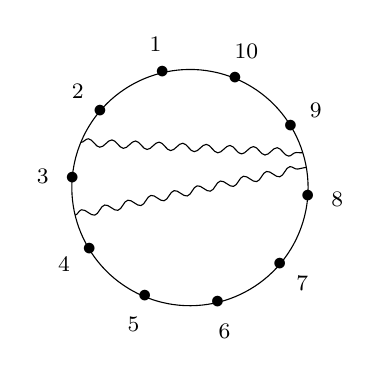
\begin{tikzpicture}[rotate=67.5,baseline=(current bounding box.east)]
	 \begin{scope}
	\drawWLD{10}{1.5}
	\drawnumbers
	\drawprop{2}{0}{8}{1}
	\drawprop{3}{0}{8}{-1}
		\end{scope}
	\end{tikzpicture} \quad ; \quad \textrm{Config 5} = 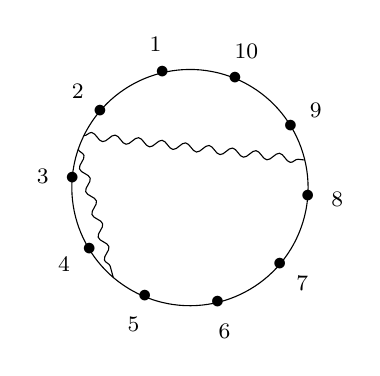
\begin{tikzpicture}[rotate=67.5,baseline=(current bounding box.east)]
	\begin{scope}
	\drawWLD{10}{1.5}
	\drawnumbers
	\drawprop{2}{-1}{8}{0}
	\drawprop{2}{1}{4}{0}
		\end{scope}
	\end{tikzpicture} \\ \textrm{Config 6} = 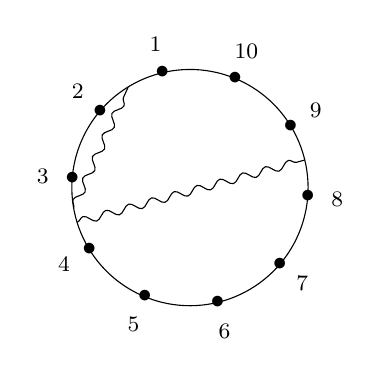
\begin{tikzpicture}[rotate=67.5,baseline=(current bounding box.east)]
	\begin{scope}
	\drawWLD{10}{1.5}
	\drawnumbers
	\drawprop{3}{1}{8}{0}
	\drawprop{3}{-1}{1}{0}
		\end{scope}
	\end{tikzpicture} \label{eq:narrowV}\eml

\begin{lem}\label{res:narrowVcancel}
Let $W_4$, $W_5$ and $W_6$ be admissible Wilson loop diagrams that are identical except for the fact that the diagram $W_i$ cotains the pair of propagators shown in $\textrm{Config i}$ above. Let $p = (i, j)$ and $q = (i, k)$ with $k = j+1$. Then \bas \lim_{(x_{p,i}x_{q, i+1} - x_{p, i+1}, x_{q, i}) \rightarrow 0} I(W_4) + \lim_{x_{r, j+3} \rightarrow 0}I(W_5) + \lim_{x_{r, k-2} \rightarrow 0}I(W_6) = 0\;.\eas \end{lem}
\begin{proof}
This proof follows similarly to the above. Write \bas x_*(W_4) = \begin{bmatrix}1 & \ldots & a &b &\ldots & c & d & 0 & \ldots \\  1 & \dots &  ae &be + f  & \ldots &0 & g & h & \ldots    \end{bmatrix}  \\ x_*(W_5) = \begin{bmatrix}1 & \ldots & a' &b' &\ldots & c' & d' & 0 & 0& \ldots \\  1 & \dots &  0&0  & \ldots &c'e' & d'e' +f' & g' & h' & \ldots    \end{bmatrix} \\ x_*(W_6) = \begin{bmatrix}1 & \ldots & 0 &0 &\ldots & a'' & b'' & c''g'' & h'' c'' + d'' & \ldots \\  1 & \dots &  e'' & f''  & \ldots &0&0 & g'' & h'' & \ldots    \end{bmatrix} \;. \eas We consider the change of variables defined by the product \bas \begin{bmatrix}1 & 0 \\ \frac{-e'}{1-e'} & \frac{1}{1-e'} \end{bmatrix} x_*(W_5)  \quad \textrm{ and } \quad \begin{bmatrix}\frac{1}{1-c''} & \frac{-c''}{1-c''} \\ 0 & 1 \end{bmatrix} x_*(W_6) \;.\eas Then the same types of calculations as in Lemma \ref{??} shows that $ \lim_{x_{r, k-2} \rightarrow 0}I(W_6)  =  \lim_{f \rightarrow 0} \frac{-1}{1-e} I(W_4) $ and $\lim_{x_{r, k-2} \rightarrow 0}I(W_5)  =  \lim_{f \rightarrow 0} \frac{e}{1-e} I(W_4) $, proving the result.
\end{proof}


%Let $\mathcal{P} = \{P_1, P_2, \dots, P_k\}$ be a collection of subsets of $\{1,2,\dots,n\}$. Let $\mathbf{x}=\{x_{i,j}\}$ be algebraically independent invertible variables. Define $M_{\mathcal{P}}(\mathbf{x})$ to be the $n \times k$ matrix having $x_{i,j}$ as its $i,j$ entry if $j \in P_i$ and $0$ otherwise.

\begin{thm}\label{res:Rado}
Let $\mathcal{P}$ be a collection of subsets, and let $\mathbf{x} = x_{i,j}$ and $\mathbf{y} = y_{i,j}$ be two sets of algebraically independent invertible variable which are related by a change of variable matrix with nonzero Jacobian. Let $M_{\mathcal{P}}(\mathbf{x})$ and $M_{\mathcal{P}}(\mathbf{y})$ be the variable valued matrices associated to $\mathcal{P}$ in the variables $\mathbf{x}$ and $\mathbf{y}$. Let $S \subset \mathbf{x}$, with $d = |\mathbf{x}| - |S|$ and consider $M' = M_{\mathcal{P}}(\mathbf{y})|_{x_{i,j} = 0; x_{i,j} \in S}$. Note that there are $d$ variables in $\mathbf{x}$ remaining. Let $G$ be the subset of $\Gr(k,n)$ consisting of row spaces of matrices obtained by evaluating the remaining $x_{i,j}$ in $M'$ at real parameters. For $I \subset \{1, \dots, k\}$, let $R_I$ be the subset of $\mathbb{R}^n$ obtained by evaluating linear combinations of the rows of $M'$ indexed by $I$ at real parameters. The following are equivalent:
\begin{itemize}
\item[(i)] For all $I \subsetneq \{1,2, \dots, k\}$ and all $j \in I^c$, $R_{I \cup j} \neq R_I$.
\item[(ii)] $\mathrm{dim}(G) = d-k$.
\end{itemize}
\end{thm}

\begin{proof}
We show that (ii) implies (i) via induction on $k$. When $k = 1$, $G$ is a parameterized subset of projective space and the result holds. Suppose that the result holds for $k = l-1$. Let $M'$ be an $n \times l$ matrix such that $R_{\{1,\dots,l\}} = R_{1,\dots,l-1}$, and suppose that $R_I \neq R_{I \cup j}$ for $j \notin I$ whenever $|I| < l$. For any subset $S \subset [k]$, let $d_S$ be the number of parameters in the $\mathbf{x}$ variables appearing in the rows of $M'$ indexed by $S$.

$G$ is spanned by an element $r$ in $G_{\{l\}}$, plus a $k-1$ plane in $G_{\{1,\dots,l-1\}} \cap \Gr(\mathbb{R}^n \perp r, k-1)$. Since $r \in R_{1, \dots, l-1}$,
%
\begin{displaymath}
\dim(G_{\{1,\dots,l-1\}} \cap \Gr(\mathbb{R}^n \perp r, k-1)) < \dim(G_{\{1,\dots,l-1\}}).
\end{displaymath}
%
\noindent
So,
%
\begin{displaymath}
\dim(G) \leq \dim(G_{\{l\}}) + (\dim(G_{\{1,\dots,l-1\}}) - 1) = d -k - 1,
\end{displaymath}
%
\noindent
and thus (ii) implies (i) when $k = l$.



To show that (i) implies (ii), suppose that $\mathrm{dim}(G) < d-k$. Then, there is some $A \in Gl(k,\mathbb{R}(\mathbf{x}))$ such that $A \cdot M'$ contains strictly fewer than $d$ parameters. Suppose that the parameter $x_{a,b}$ is eliminated in $A \cdot M'$. We claim that $R_{[k] \setminus a} = R_{[k]}$.

\begin{itemize}
\item Take $a$-th row of a specific evaluation of $M'$, suppose it is not contained in $R_{[k] \setminus a}$.
\item
\end{itemize}
\end{proof}

\begin{eg}
Consider
\begin{displaymath}
\begin{bmatrix}
1 & p_1 & p_2 & p_3 & p_4 & 0 & 0 \\
1 & p_1 p_5 & p_2 p_5 + p_6 & 0 & 0 & p_7 & p_8 \\
1 & 0 & 0 & p_9 & p_{10} & p_{11} & p_{12}
\end{bmatrix}
\end{displaymath}
can kill off 9
\end{eg}

\begin{rmk}
remark: this is a rado theorem thing.
\end{rmk}

\end{appendices}








\end{document}
